% Compile with XeLaTeX (tectonic) — uses system fonts for Cyrillic support
\documentclass[11pt,letterpaper]{article}
\usepackage{fontspec}
\setmainfont{Times New Roman}
\usepackage{amsmath}
\usepackage{booktabs}
\usepackage[letterpaper,margin=1in]{geometry}
\usepackage{caption}
\usepackage{multirow}
\usepackage{natbib}
\usepackage{graphicx}
\usepackage{float}
\usepackage[hidelinks]{hyperref}
\captionsetup{font=small,labelfont=bf}
\usepackage{worldflags}
\usepackage{tikz}
\usetikzlibrary{shapes.geometric, arrows.meta, positioning, calc}
\newcommand{\flagENG}[1][5mm]{\begin{tikzpicture}[x=#1,y=#1,baseline=-0.4ex]\fill[white](0,0)rectangle(1,.6);\fill[red!88!black](.42,0)rectangle(.58,.6);\fill[red!88!black](0,.26)rectangle(1,.34);\draw[black,line width=.15pt](0,0)rectangle(1,.6);\end{tikzpicture}}
\newcommand{\flagSCO}[1][5mm]{\begin{tikzpicture}[x=#1,y=#1,baseline=-0.4ex]\fill[blue!55!black!92](0,0)rectangle(1,.6);\begin{scope}\clip(0,0)rectangle(1,.6);\draw[white,line width=.12*#1](0,0)--(1,.6);\draw[white,line width=.12*#1](0,.6)--(1,0);\end{scope}\draw[black,line width=.15pt](0,0)rectangle(1,.6);\end{tikzpicture}}
\newcommand{\flagCUW}[1][5mm]{\begin{tikzpicture}[x=#1,y=#1]\fill[blue!75!black!92](0,0)rectangle(1,.6);\fill[yellow!92!orange](0,.13)rectangle(1,.21);\fill[white](.17,.43)circle(.045);\fill[white](.30,.30)circle(.03);\draw[black,line width=.15pt](0,0)rectangle(1,.6);\end{tikzpicture}}

\title{\textbf{Forecasting the 2026 FIFA World Cup: A Market-Calibrated Poisson--Elo Model and the Information Each Result Reveals}}
\author{Avralt-Od Purevjav\\ \small Washington, DC, USA \\ \small \texttt{avraltod@gmail.com}}
\date{Pre-kickoff version, \today}

\begin{document}
\maketitle

\begin{abstract}
\noindent This paper documents a forecasting framework I built to predict all 104 matches of the 2026 FIFA World Cup, the first edition with 48 teams. The objective is to maximize an entry's expected score in a private prediction pool that awards 3 points for an exact scoreline, 2 for the correct result and goal difference, and 1 for the correct result, so the target quantity is an expected-value-optimal scoreline and not the most likely winner. The group-stage forecasts derive from bookmaker odds collected four days before kickoff, margin-stripped and fitted to independent Poisson goal distributions, and the knockout forecasts use World Football Elo ratings adjusted for confirmed squad injuries and host advantage. I then simulate 200{,}000 full tournaments to stress-test the bracket. Because a knockout prediction can score only if the named team actually occupies its bracket slot, I optimize the picks for \emph{slot emergence}, the joint probability of reaching and winning a slot, following the expected-pool-score principle of the office-pool literature and applying it to the 48-team format's constrained third-place allocation. This criterion overturned three knockout picks, and two of them survive a full sensitivity sweep over the framework's hand-set constants. The model forecasts Spain as champion in 27.4 percent of simulations, defeating Argentina (18.6 percent) in the final, with France (14.8 percent) third. The paper's central pre-registered analysis treats this static forecast as a baseline and studies how it revises as the tournament is played. After each result I fix the played matches and re-simulate the rest, which updates every team's probability of reaching each stage, and I measure the information each result carries by the Kullback--Leibler divergence between the champion distribution before and after it. I register the hypothesis that this information is highly uneven across the 104 matches, near zero through most of the group stage and concentrated at the eliminations of likely champions. All predictions are locked before kickoff, so the forecast trajectory is an out-of-sample record, and all data and code are retained for that evaluation.

\medskip
\noindent\textbf{Keywords:} association football, betting odds, Poisson model, Elo ratings, Monte Carlo simulation, FIFA World Cup
\end{abstract}

\begin{center}
\rule{0.6\textwidth}{0.4pt}
\end{center}

% ---- Update log stamped on the first page ----
\begin{center}
\footnotesize\itshape
Update log --- forecast built 7 June 2026 from bookmaker odds collected 5--7 June;
Group~K recalibrated to prediction-market prices the evening of 7 June;
squad and injury news monitored through 9 June, entry confirmed unchanged so far;
predictions lock at the 11 June kickoff. Code and data timestamped for the out-of-sample record.
\end{center}

% ---- Mongolian abstract: commented out for now (re-enable by removing \iffalse ... \fi) ----
\iffalse
\begin{quotation}
\small\noindent\textbf{Хураангуй.} Энэхүү өгүүлэлд 2026 оны ФИФА-гийн Дэлхийн аварга шалгаруулах тэмцээний нийт 104 тоглолтыг урьдчилан таамаглах загварыг баримтжуулав. Найз нөхдийн дунд явагддаг мөрийтэй таамаглалын онооны журам нь зөв үр дүнгээс илүү яг оноог өндрөөр үнэлдэг тул судалгааны зорилт нь хамгийн магадлалтай яг тоог олоход чиглэв. Хэсгийн тоглолтуудын таамаглалыг бухмэйкерийн ханшид суурилсан Пуассоны загвараар, шигшээ шатны таамаглалыг гэмтлийн мэдээ болон талбайн давуу талаар залруулсан Эло үнэлгээгээр гаргав. 200{,}000 удаагийн Монте-Карло симуляциар таамаглалын хүснэгтийг шалгаж, дөрвөн сонголтыг өөрчлөв. Загварын таамаглалаар Испани улс финалд Аргентиныг хожиж аварга болно (симуляцийн 27.4\%).

\smallskip
\noindent\textbf{Түлхүүр үгс:} хөлбөмбөг, бухмэйкерийн ханш, Пуассоны загвар, Эло үнэлгээ, Монте-Карло симуляци
\end{quotation}
\fi

\section{Introduction}

The 2026 FIFA World Cup runs from June 11 to July 19, 2026 across Canada, Mexico, and the United States, and it expands the tournament to 48 teams, 12 groups, and a new Round of 32 in which the eight best of the twelve third-placed teams advance. The expansion roughly triples the combinatorial complexity of bracket prediction relative to the 32-team format, because a knockout matchup now depends not only on which teams win their groups and finish second but on a constrained allocation of third-placed teams to predetermined bracket slots. A forecaster who must name every match before the tournament starts therefore faces a harder problem than in any previous edition.

The forecasting problem I address is shaped by its application. I participate in a long-running prediction pool among friends in which each participant submits a complete tournament forecast, every group-match scoreline and the full knockout bracket, before the opening match. The pool awards 3 points for an exact scoreline, 2 for the correct result and goal difference, and 1 for the correct result only, and my objective is to maximize the expected point total of my entry under that rule. This is a deliberate scoping choice, because a pool is ultimately a rank-order contest, and the game-theoretic pool literature shows that maximizing expected score and maximizing the probability of finishing first can diverge when rivals cluster on consensus picks \citep{clairletscher2007}. Section~\ref{sec:objective} returns to why per-match additive scoring attenuates that divergence without eliminating it.

The problem of choosing a bracket entry to maximize expected pool score is not new. \citet{kaplangarstka2001} give an exact dynamic-programming solution for March Madness office pools, and \citet{clairletscher2007} extend it with opponent modeling. What the 2026 format adds is structure those analyses did not face, because twelve groups feed a Round of 32 through a constrained third-place allocation table, and this makes the probability that a team \emph{occupies} a given slot both harder to compute and more decision-relevant. My slot-emergence criterion is a Monte Carlo estimate of the Kaplan--Garstka objective adapted to that structure.

Three further results motivate the design. First, bookmaker odds are among the strongest publicly available probability forecasts for football matches \citep{strumbelj2014, leitner2010}, although hybrid statistical models have matched or beaten them in recent tournaments \citep{groll2018, groll2019}. Second, independent Poisson distributions calibrated to match-level win probabilities reproduce observed scoreline frequencies well at the international level \citep{maher1982, dixoncoles1997}. Third, ratings systems give serviceable strength estimates where market odds do not yet exist, such as hypothetical knockout pairings \citep{hvattum2010, elo1978, constantinou2019}. Bookmaker-consensus methods that simulate tournaments from market-implied abilities \citep{zeileis2018} are the main alternative, and I use Elo for the knockout stage because the market had not yet priced those pairings at submission time, not because Elo is superior.

In this paper I combine these components and add a tournament-structure layer, a Monte Carlo simulation that scores candidate bracket entries by slot emergence. The model forecasts Spain as champion in 27.4 percent of 200{,}000 simulated tournaments, ahead of Argentina at 18.6 percent and France at 14.8 percent, and it produces a submitted bracket in which Spain defeats Argentina in the final. The slot-emergence criterion overturns three of the 31 knockout picks that a head-to-head rule would have made, and two of the three survive a sensitivity sweep over every hand-set constant in the framework.

The static forecast is only the starting point. The paper's central contribution is to treat it as a baseline, a prior fixed before any match is played, and to study how the forecast revises as results arrive. After each match I condition on the played results and re-simulate the rest, which moves every team's probability of reaching each stage, and I measure the information each result carries by the divergence between the champion distribution before and after it. Because the format lets strong teams advance even after an early loss, I expect most group-stage matches to carry almost no information and the forecast to be reshaped late, at the eliminations of likely champions. This turns a one-shot prediction into a study of probability revision under a known information-arrival schedule, and because every prediction is locked before kickoff the resulting trajectory is an honest out-of-sample record.

The rest of the paper is organized as follows. Section~2 describes the data, Section~3 the methodology, and Section~4 the results, including the pre-registered forecast-evolution study, and Section~5 discusses the forecast, its objective, and the ways it can fail.

\section{Data}

I collected four datasets on June 5--7, 2026, four days before the opening match (Table~\ref{tab:data}).

\begin{table}[ht]
\centering\small
\caption{Data sources (collected June 5--7, 2026).}
\label{tab:data}
\begin{tabular}{p{3.4cm}p{5.2cm}p{5.6cm}}
\toprule
Dataset & Source & Coverage \\
\midrule
Match odds (1X2) & bet365, FanDuel, Betfair, DraftKings, and odds aggregators & 48 of 72 group fixtures with published lines; remaining 24 (mostly matchday 3) estimated from Elo \\
Outright winner odds & Multi-bookmaker consensus & Top 15 favorites \\
Elo ratings & World Football Elo Ratings (eloratings.net) & All 48 qualified teams \\
Squad news & ESPN, Sky Sports, Goal.com injury trackers & Confirmed tournament-eve injuries and June friendly results \\
\bottomrule
\end{tabular}
\end{table}

I incorporate several squad facts as rating adjustments, including Brazil without Rodrygo (anterior cruciate ligament), the Netherlands without Xavi Simons, Japan without Kaoru Mitoma, Croatia in poor warm-up form, and a minor deduction for Spain (Fermín López). I take the fixture list, kickoff times, venues, and the official third-place allocation table from the tournament schedule.

\section{Methodology}\label{sec:method}

\subsection{From odds to probabilities}

Decimal odds $o_H, o_D, o_A$ for a home win, draw, and away win embed a bookmaker margin. Fair probabilities were recovered by basic normalization,
\begin{equation}
p_r = \frac{1/o_r}{\sum_{s \in \{H,D,A\}} 1/o_s}, \qquad r \in \{H,D,A\},
\end{equation}
Basic normalization is a deliberate simplification: \citet{strumbelj2014} showed it is generally inferior to Shin's method, which corrects the favorite--longshot bias in the margin's distribution. The simplification is acceptable for the present decision problem because the target is the expected-value-optimal scoreline, not a staking probability, and re-de-vigging the 24 fixtures with published lines under Shin's method changes only 2 of the 24 resulting picks; it would not be acceptable if the forecasts were used for staking. For the 24 fixtures without published lines, probabilities were estimated from Elo differences using the win expectancy in Section~\ref{sec:elo}. The Poisson fit reproduces the market probabilities closely, with a mean root-mean-square residual across the home, draw, and away targets of 0.003 and the goal-sum constraint binding on only 6 of the 72 fixtures.

\subsection{Poisson scorelines}

Goals for the home and away side are modeled as independent Poisson variables with rates $\lambda_h, \lambda_a$ \citep{maher1982}; the bivariate-Poisson tradition \citep{karlis2003} and the low-score dependence correction of \citet{dixoncoles1997} relax this independence, and Section~\ref{sec:audit} tests the latter on the decision metric. Dynamic state-space variants \citep{koopmanlit2015} additionally let team strength vary over time, which the frozen-strength design here deliberately forgoes. For each match the rate pair was fitted by grid search to reproduce the market's outcome probabilities,
\begin{equation}
(\hat\lambda_h, \hat\lambda_a) \;=\; \underset{\lambda_h,\lambda_a}{\arg\min} \sum_{r \in \{H,D,A\}} \bigl(\pi_r(\lambda_h,\lambda_a) - p_r\bigr)^2
\quad \text{s.t.} \quad 1.6 \le \lambda_h + \lambda_a \le 3.4,
\end{equation}
where $\pi_r$ is the outcome probability implied by the Poisson pair and the constraint reflects historical World Cup scoring rates. The pool scores a prediction in three tiers, awarding 3 points for the exact score, 2 for the correct result and goal difference, and 1 for the correct result, so the expected value of a pick $(h,a)$ with result $r$ and goal difference $g$ is
\begin{equation}
\mathrm{EV}(h,a) \;=\; P(h,a) \;+\; P\bigl(\text{result}=r,\ \text{GD}=g\bigr) \;+\; P\bigl(\text{result}=r\bigr),
\label{eq:ev}
\end{equation}
because the exact score earns all three tiers, the right goal difference earns the lower two, and the right result earns the lowest. The published prediction maximizes Equation~\eqref{eq:ev} over all scorelines. The goal-difference tier shapes the picks in two ways. For a favorite the optimal pick is a one-goal margin such as 1--0, because winning by one is the most common margin and the middle tier rewards getting the margin right rather than only the winner. For an evenly matched fixture the optimal pick is a 1--1 draw, because every drawn scoreline shares goal difference zero, so a draw prediction collects the 2-point tier on any drawn result and not only on an exact 1--1. The entry therefore contains a small number of draws, on the most balanced fixtures, alongside the one-goal favorites that dominate the rest.

The same expected value can be read pick by pick, and it makes the structure of the entry concrete (Figure~\ref{fig:pickvalue}). Each of the 104 predictions carries an expected-points value between 0.65 and 1.37 under the three-tier rule, averaging 0.99, and the spread is informative: a confident pick against a weak side, such as England's 2--0 over Ghana at 1.37 expected points, is worth roughly twice the most evenly matched game, such as the 1--1 draw between Turkey and the United States at 0.68. The group stage sums to 72.0 expected points and the knockout stage to 31.0 conditional on the predicted matchups occurring. The figure is also the natural scoreboard for the live evaluation, because each realized result can be set against the expected value its pick carried.

\begin{figure}[ht]
\centering

\includegraphics[width=0.92\textwidth]{figs/fig_pickvalue.pdf}
\caption{Expected points per pick for all 104 predictions, sorted, under the pool's three-tier rule (group orange, knockout blue). Confident picks against weak teams sit highest and the most even games lowest; the mean is 0.99 points per game. Knockout values are conditional on the predicted matchup occurring.}
\label{fig:pickvalue}
\end{figure}

\subsection{Knockout model}\label{sec:elo}

No market odds exist for hypothetical knockout pairings, so knockout matches use Elo win expectancy \citep{elo1978, hvattum2010},
\begin{equation}
E_{AB} = \bigl(1 + 10^{-\Delta/400}\bigr)^{-1}, \qquad \Delta = R_A - R_B,
\end{equation}
with a draw component for the 90-minute result, $p_D = 0.30\, e^{-|\Delta|/700}$, and $p_H = E_{AB} - p_D/2$. The draw component's constants are assumptions, not estimates: 0.30 anchors the equal-strength draw rate near the historical international rate, and the 700-point decay is a smoothness choice; neither is fitted to data, and Section~\ref{sec:robust} reports how the bracket decisions respond when the rating inputs they interact with are perturbed. Ratings $R$ are the June 2026 Elo values adjusted for confirmed injuries (Brazil $-20$, Netherlands $-15$, Japan $-10$, Croatia $-10$, Spain $-5$) and host advantage ($+40$ for Canada, Mexico, and the United States at home venues, decaying to $+20$ in the quarter-finals onward); these too are judgment values, examined in the same sensitivity sweep. Where the modal 90-minute result is a draw, the higher-rated side is entered as winner after extra time or penalties.

\subsection{Monte Carlo tournament simulation}

The full tournament was simulated 200{,}000 times. Each iteration (i) samples every group match scoreline from its fitted Poisson pair; (ii) resolves group tables by points, goal difference, goals scored, head-to-head result, and random draw; (iii) ranks the twelve third-placed teams by points, goal difference, goals scored, and a random tiebreak, takes the best eight, and assigns their groups to the eight third-place bracket slots by backtracking bipartite matching against the official allocation table, in which each slot admits only a fixed subset of groups and slots are filled in order with the first feasible group; if the best eight admit no complete matching the search retries with the ninth-ranked group substituted for the eighth, which resolves every infeasible case that arises; and (iv) plays all 31 knockout matches as Elo-weighted Bernoulli draws. With $N = 200{,}000$, the Monte Carlo standard error of an estimated probability $p$ is $\sqrt{p(1-p)/N} \le 0.11$ percentage points. Beyond the headline probabilities of Section~4, the simulation yields each team's full distribution over exit stages; Appendix~\ref{app:survival} reports these survival distributions for sixteen teams.

\subsection{Slot-emergence optimization}\label{sec:slot}

A knockout entry scores only if the named team contests the corresponding real match. The relevant decision quantity for bracket slot $s$ is therefore not head-to-head win probability but
\begin{equation}
T^\ast_s \;=\; \arg\max_T \; P_{\mathrm{sim}}\bigl(T \text{ occupies and wins slot } s\bigr),
\label{eq:slot}
\end{equation}
estimated from the simulation. Criterion~\eqref{eq:slot} can disagree with head-to-head strength, because a stronger team that frequently wins its group exits the predicted slot entirely, while a weaker team with a stable path to the slot accumulates more expected points there.

\subsection{Conditional updating and the information content of a result}\label{sec:updating}

The pre-tournament simulation of Section~\ref{sec:elo} is a baseline, the forecast before any match is played, and I treat it as the prior at time zero. Each result that arrives is new information, and I update the forecast by conditioning. After a set of matches is played I fix their realized outcomes and re-simulate only the remaining matches, holding every still-alive team at its pre-tournament strength. This is conditioning, not learning: the played results reshape which teams occupy which bracket slots and which paths are still open, but I do not re-estimate any team's strength from its performance, so the update is the change in the bracket's structure rather than a change in beliefs about ability. Freezing strengths could in principle suppress group-stage information, because a dominant early performance that ought to raise a team's strength registers only through the bracket. I therefore checked the choice directly, re-running the 2018 and 2022 evolution with Elo strengths updated after each match by the standard rule with a goal-difference multiplier: the group-stage share of total information rises only from 17 to 20 percent in 2018 and from 21 to 22 percent in 2022, and the knockout stage still carries about four-fifths of the information under both models. The strength-updating channel is real but small, and the concentration in the knockouts is robust to whether it is included. After each result the conditional simulation gives an updated probability that each team reaches each stage, and the sequence of these snapshots is the forecast's trajectory through the tournament.

The natural way to measure how much a result moved the forecast is the information it carried. Let $q$ be the champion distribution after a result and $p$ the distribution before it. The Kullback--Leibler divergence
\begin{equation}
D(q \parallel p) \;=\; \sum_{\text{teams } t} q_t \log_2 \frac{q_t}{p_t}
\label{eq:kl}
\end{equation}
measures, in bits, how far the forecast moved, and it is the central quantity of the live study. A favorite winning as expected carries almost no information and leaves $D$ near zero, while a favorite eliminated carries a large amount and produces a spike. I pre-register the hypothesis that the information is highly uneven across the 104 matches, concentrated at eliminations and at the matchday-three fixtures that decide group order, and close to zero through most of the group stage, because the format lets the best teams advance even after an early loss.

These measures are not new, and the contribution here is their application to a pre-registered live tournament record, not the measures themselves. The per-result divergence in Equation~\eqref{eq:kl} is the relative entropy that underlies the logarithmic scoring rule of \citet{gneiting2007}, and the expected version introduced as pivotality in Section~\ref{sec:pivotality} is the mutual information between a result and the champion's identity, which is the same quantity the sabermetric literature calls win-probability-added or leverage \citep{tango2007}. The belief-path object the trajectory traces, the cumulative movement of a forecast as uncertainty resolves, is studied formally by \citet{ely2015} as suspense and surprise. I use these established tools to instrument a forecast over a real tournament; the novelty I claim is the pre-registered record and the slot-emergence decision rule of Section~\ref{sec:slot}, not the information measures.

\section{Results}

\subsection{Tournament-level forecasts}

Table~\ref{tab:champ} reports champion, finalist, and semi-finalist probabilities. Spain is the modal champion at 27.4\%, ahead of Argentina at 18.6\% and France at 14.8\%, and the predicted Spain--Argentina final is the single most likely pairing at 10.8\% of simulations.\footnote{This is the original locked forecast. Two later numbers in the paper differ by about a percentage point: the pre-deadline Group~K recalibration of Section~\ref{sec:postscript} revises Spain to 26.8\%, and Monte Carlo variation across runs is about 0.5~pp (Section~\ref{sec:robust}). I report the original 27.4\% as the headline and the recalibrated 26.8\% wherever the recalibrated model is the explicit subject; the two are the same forecast before and after that single localized update.} The forecast is consistent with the outright betting market, which priced Spain as favorite at decimal odds near 5.5.

\begin{table}[ht]
\centering\small
\caption{Simulated tournament probabilities, top eight teams ($N$ = 200{,}000; standard errors $\le$ 0.11 pp).}
\label{tab:champ}
\begin{tabular}{lccc}
\toprule
Team & Champion & Finalist & Semi-finalist \\
\midrule
Spain          & 27.4\% & 39.0\% & 51.8\% \\
Argentina      & 18.6\% & 30.9\% & 44.3\% \\
France         & 14.8\% & 25.2\% & 43.6\% \\
England        &  7.3\% & 15.1\% & 29.0\% \\
Portugal       &  4.2\% &  9.8\% & 18.6\% \\
Colombia       &  4.1\% &  9.5\% & 18.4\% \\
Brazil         &  3.6\% &  8.7\% & 20.3\% \\
Netherlands    &  2.7\% &  6.7\% & 16.6\% \\
\bottomrule
\end{tabular}
\end{table}

\begin{figure}[ht]
\centering

\includegraphics[width=0.92\textwidth]{figs/fig1_champion_dist.pdf}
\caption{Champion probability distribution across 200{,}000 simulated tournaments. Spain (blue) is the modal champion yet fails to win in 72.6\% of simulations; Portugal (orange) is discussed in Section~\ref{sec:portugal}. The 36 teams outside the top twelve jointly retain a 9.7\% champion share.}
\label{fig:champdist}
\end{figure}

The distribution in Figure~\ref{fig:champdist} is heavy-tailed in a way the headline forecast obscures, because the modal champion is more likely wrong than right, and nearly a tenth of the probability mass sits outside the twelve named contenders. This is a property of tournament football and not of the model, because knockout formats convert small per-match upset probabilities into large aggregate ones.

\subsection{Simulation-driven bracket revisions}

Applying criterion~\eqref{eq:slot} to the greedily constructed bracket overturned three of the 31 knockout entries, and it routed an even group-stage call toward the structurally better side (Table~\ref{tab:revisions}). That group-stage case needs one clarification, because the Turkey--United States fixture is a near-tie whose expected-value-optimal scoreline under the three-tier rule is a 1--1 draw, which is what the entry submits; the slot-emergence analysis then assigns the group-winner position to the United States for better bracket structure. Because the pool scores each match independently, this routing choice shapes the predicted path but not the entry's points, so the scoreline and the routing are two separate decisions that need not agree. The Belgium revision is the largest, because Turkey, the head-to-head favorite in the predicted Round-of-16 pairing, reaches that slot in only 14.3\% of simulations, since its path requires first winning a tight Group D and then a Round-of-32 tie, while Belgium's route through Group G is substantially safer. The Croatia--Portugal case illustrates the subtler failure mode, because Portugal is the stronger side and yet it too often wins Group K outright across the 200{,}000 simulations and never contests the predicted slot at all.

\begin{table}[ht]
\centering\small
\caption{Bracket entries revised by slot-emergence analysis. For the three knockout rows, percentages are the probability that the named team occupies and wins the slot; the group-stage row submits the even fixture's expected-value-optimal 1--1 draw and routes the resulting tied group to the United States for bracket structure, a routing choice the pool scores independently of the submitted scoreline.}
\label{tab:revisions}
\begin{tabular}{llccc}
\toprule
Slot & Revision & Original & Revised & Gain \\
\midrule
Group D, match 59 & Turkey 1--1 USA (EV-optimal draw), routed to USA & \multicolumn{2}{c}{tied call (36.3\% / 36.3\%)} & --- \\
Round of 32, M78 & Ecuador $\to$ Norway & 20.5\% & 24.5\% & $+4.0$ pp \\
Round of 32, M83 & Portugal $\to$ Croatia & 25.1\% & 27.5\% & $+2.4$ pp \\
Round of 16, M94 & Turkey $\to$ Belgium & 14.3\% & 23.9\% & $+9.6$ pp \\
\bottomrule
\end{tabular}
\end{table}

The three overturned picks understate the criterion's importance, because the right way to value slot emergence is over the whole bracket and against the baseline a naive forecaster would actually use. Scored across all 31 knockout matches, a slot-emergence entry earns 11.5 expected knockout points, against 4.3 for an entry that fills each slot with the strongest team that could reach it. The gap is the Portugal paradox at scale: the strongest reachable team for a deep slot is usually a giant who arrives there too rarely to score, so an entry built on raw strength leaves most of its knockout points unclaimed. The advantage is not specific to the 2026 draw either; repeating the comparison on four tournaments with team strengths randomly perturbed by 80 Elo points gives a slot-emergence margin over the strongest-team entry of between 5.1 and 6.9 points in every case. Against a less naive baseline that fills each slot with its most likely \emph{occupant}, however, slot emergence adds only about 0.2 points, so almost all of the value comes from routing the pick toward a slot the team is likely to occupy, and the marginal refinement of also conditioning on winning that slot is small. The decision-relevant lesson is the first comparison: committing one name per slot, strength is the wrong objective and reachability is most of the right one.

\subsection{Robustness of the revisions}\label{sec:robust}

Two objections apply to Table~\ref{tab:revisions} and deserve direct treatment. First, the revisions are in-model preferences, because the same simulation that produced the original picks is asked whether it prefers alternatives, so they constitute internal consistency and not external validation, and only the realized tournament can provide the latter. Second, the deciding margins of 2.4 to 9.6 pp must be compared not against the Monte Carlo sampling error of 0.11 pp, which is negligible, but against the uncertainty of the hand-set rating inputs, which is far larger and not formally quantified.

A one-at-a-time sensitivity sweep addresses the second objection. I perturb each hand-set constant across a wide range, scaling the injury adjustments by 0, 0.5, 1.5, and 2 and setting host advantage to 0, 20, and 60 points, and I re-run the simulation at 20{,}000 iterations per configuration, which gives a standard error near 0.45 pp on each gap. The Norway--Ecuador gap is 3.5 pp in every configuration and the Belgium--Turkey gap stays between 8.3 and 9.1 pp, so these two revisions are insensitive to the framework's judgment inputs. The Croatia--Portugal gap remains positive in all configurations but shrinks from 3.0 pp with injuries off to 0.8 pp with injuries doubled, because Croatia carries one of the adjustments, so it is sign-stable but small and I report it as the least secure of the three. The champion forecast is unaffected throughout, and Spain wins in every configuration at between 26.8 and 27.9 percent. The draw-model constants are excluded from the sweep for cause rather than omission: because the knockout winner is sampled with probability $p_h + p_d/2$, which equals the raw Elo win expectancy regardless of how the draw mass is set, the constants $0.30$ and the 700-point decay cancel in every knockout and touch only the 24 Elo-estimated group fixtures, leaving the champion forecast unmoved. Because one-at-a-time perturbation can miss interactions, I also drew ten joint configurations of the injury scaling and host magnitude at random: Spain's champion probability stayed within a 0.8-point band of 26.2 to 27.1 percent, and all three slot-emergence revisions remained sign-stable in every configuration.

The aggregate stake is worth stating plainly. Summed over the three slots, the revisions raise the expected number of correctly named slot winners by about 0.16, which is roughly one extra correct knockout call every six tournaments. The framework's value lies less in any single revision than in the systematic check, because without the simulation all three head-to-head favorites would have been entered, and two of those entries are robustly dominated.

\subsection{Final forecast}

The submitted bracket has Spain defeating Argentina 1--0 in the final at MetLife Stadium on July 19, with France third over England. Semi-finals: Spain over France and Argentina over England, both 1--0. The complete match-level forecast (72 group scorelines and 31 knockout entries) accompanies this paper as the official pool submission sheet.

Figure~\ref{fig:finaldist} shows the fitted scoreline distribution for the predicted final ($\hat\lambda_{\mathrm{ESP}} = 1.25$, $\hat\lambda_{\mathrm{ARG}} = 1.00$). The modal pick, 1--0, carries only 13.2\% probability; the five most likely scorelines together cover barely half the distribution. Exact-score forecasting is intrinsically low-hit-rate even when the model is well calibrated, which is why the pool strategy optimizes the \emph{sum} of many small edges rather than any single confident call.

\begin{figure}[ht]
\centering

\includegraphics[width=0.62\textwidth]{figs/fig3_final_scorelines.pdf}
\caption{Fitted Poisson scoreline distribution for the predicted final, Spain vs.\ Argentina. The orange box marks the submitted prediction (1--0), which carries only 13.2\% probability; no single scoreline is much more likely.}
\label{fig:finaldist}
\end{figure}

\subsection{Forecast evolution: a pre-registered live study}\label{sec:evolution}

The results to this point describe a single static forecast, but the more interesting object is how that forecast moves as the tournament is played, and this is the paper's central pre-registered analysis. The method is the conditional updating of Section~\ref{sec:updating}. The baseline is the pre-tournament distribution of Table~\ref{tab:champ}, with Spain at 26.9 percent, and after each of the 104 matches I re-condition the forecast and record both the updated champion probabilities and the information the result carried, in bits, from Equation~\eqref{eq:kl}. Figure~\ref{fig:trajectory} is the recording instrument: the upper panel traces each contender's champion probability from the baseline on the left to the realized outcome on the right, where the champion's probability reaches one and every other team's reaches zero, and the lower panel shows the information content of each match. All predictions are locked, so this trajectory is an out-of-sample record rather than a fitted curve.

I register three hypotheses before the tournament. First, the information is concentrated, and a small number of matches account for most of the total movement, while most group-stage games leave the forecast nearly unchanged. Second, the largest spikes coincide with eliminations of high-probability teams, because removing a likely champion redistributes a large mass of probability at once. Third, the information arrives late, rising through the knockout rounds, so that the forecast is reshaped more in the final fortnight than across the entire group stage.

To verify that the recording machinery behaves as registered, I ran it once as a dress rehearsal, treating a single simulated tournament as if it were the real one and feeding its 104 results through the pipeline in order. Figure~\ref{fig:trajectory} shows the result. The synthetic run reproduces all three hypothesized patterns. The information is concentrated, because the ten most informative matches carry 69 percent of the total; the information arrives late, because the group stage accounts for only 19 percent of the movement against 81 percent for the knockouts; and the largest single spike, 0.52 bits, falls on a semi-final that eliminates a likely finalist. The champion probabilities stay nearly flat through the group stage, then move sharply once elimination begins, with the eventual champion's probability climbing from the low twenties to one over the final two weeks. This is a demonstration on simulated data and not a forecast of the real tournament, but it confirms that the instrument measures what it is meant to. The realized trajectory will confirm or refute the same three hypotheses on real results, and the data, the conditional-simulation code, and the per-match information series are retained for that evaluation.

\begin{figure}[ht]
\centering

\includegraphics[width=0.94\textwidth]{figs/fig_trajectory_demo.pdf}
\caption{Illustrative dress rehearsal of the live study on one simulated tournament (not the real forecast). Upper panel: each contender's champion probability, traced from the pre-tournament prior on the left to the realized outcome on the right, flat through the group stage and moving sharply once eliminations begin. Lower panel: the information content of each result in bits (Equation~\ref{eq:kl}), orange for group matches and blue for knockouts, near zero through the group stage and spiking at knockout eliminations. The same figure will be regenerated on real results after each matchday.}
\label{fig:trajectory}
\end{figure}

\subsection{Model against market: a benchmarked trajectory}\label{sec:market}

The forecast does not revise in a vacuum, because a liquid prediction market revises its own champion odds on the same results, and the market is the natural benchmark for whether the model's revisions are sound. Alongside each conditional update I record the market's champion distribution from Polymarket, normalized to remove the small overround, so the live study produces two probability-revision trajectories rather than one. The comparison is informative precisely because the model and the market are built from different information. The group-stage probabilities of this model are recovered from match odds, so on the group stage the two should agree, but the model's knockout tier is Elo while the market aggregates the views of traders, so any disagreement in the champion odds comes from how the two treat the knockout stage.

At the baseline the two disagree in a specific and interpretable way (Figure~\ref{fig:marketbase}). The model places Spain at 26.9 percent against the market's 15.6 percent and Argentina at 17.9 against 8.6 percent, and it places less weight than the market on England, Brazil, and Germany. The model's champion distribution is therefore more concentrated on the top two teams than the market's, because the Elo win-expectancy of Section~\ref{sec:elo} lets a strong team march through a six-match knockout path with compounding probability, while the market prices in more of the squad-rotation, injury, and single-match variance that can end such a run. This is consistent with the literature in which betting markets are hard to beat \citep{strumbelj2014, hvattum2010} and bookmaker-consensus methods are the standard tournament benchmark \citep{zeileis2018}, and it locates the model's distinctive claim cleanly: the model is a bet that the two strongest teams convert their strength into a title more reliably than the market expects.

I do not resolve this disagreement here, because the tournament resolves it. I pre-register two questions for the live study. First, whether the two trajectories converge as results arrive, and which one moves toward the other, since convergence of the market toward the model would suggest the model's early concentration was justified, while the reverse would suggest it was overconfidence. Second, whether the model or the market revises first at the moment of a major elimination, measured by which trajectory shows the larger one-match move when a likely champion falls. Both trajectories are recorded after every match, and Figure~\ref{fig:trajectory} will carry the market line beside the model line in the final version.

\begin{figure}[ht]
\centering

\includegraphics[width=0.72\textwidth]{figs/fig_market_baseline.pdf}
\caption{Model and market champion odds at the baseline, before any match is played. The model (blue) is more concentrated on Spain and Argentina, while the market (orange) spreads more probability to England, Brazil, and Germany. The disagreement comes entirely from the knockout stage, because the model's group-stage probabilities are themselves recovered from market odds.}
\label{fig:marketbase}
\end{figure}

\subsection{Out-of-sample validation on 2018 and 2022}\label{sec:backtest}

A forecast is only as trustworthy as its calibration, and the only way to check calibration is against realized results. I therefore ran the pipeline on the two most recent World Cups, the 2018 tournament in Russia and the 2022 tournament in Qatar, using pre-tournament Elo ratings as the probability source for every match, since per-match betting odds are not archived for those tournaments at the coverage I have for 2026. Each tournament has 64 matches, which gives 128 out-of-sample matches in total. I emphasize that this tests the Elo-based version of the pipeline, because the 2026 group stage draws on sharper market odds that the historical exercise cannot replicate, so the backtest is a lower bound on the calibration the live model should achieve.

The probabilities are roughly calibrated and carry modest skill, though two tournaments support no stronger statement. Across the 128 matches the model's multiclass Brier score beats a uniform baseline by 10 percent and its ranked probability score \citep{constantinou2012} by 11 percent, the latter splitting into 16 percent in 2018 and 5 percent in 2022; the uniform baseline is weak, and per-match historical market odds were not available to me as the more demanding benchmark, so these figures establish informativeness, not an edge over the market. The reliability of the top pick rises roughly monotonically with confidence (Figure~\ref{fig:backtest}, left): the matches called in the 60 and 70 percent bins were won 56 and 66 percent of the time. But each bin holds only 8 to 32 matches, the 95 percent intervals span 20 to 30 percentage points, and the champion-level comparison is two data points, so I read the backtest as a sanity check that the engine is not grossly miscalibrated, not as a validation. The 2022 tournament was harder for every forecaster, because it produced an unusual run of upsets, with Saudi Arabia beating Argentina, Japan beating both Germany and Spain, and Morocco reaching the semi-finals; that the model's apparent skill was lower that year is consistent with the tournament rather than the method, but with one tournament per claim this attribution is itself untestable.

At the champion level the model and the market are comparably imperfect, which is what the literature predicts (Figure~\ref{fig:backtest}, right). In 2018 the model gave the eventual champion France a 7 percent chance against the market's 13 percent, so the market was closer, while in 2022 the model gave Argentina 22 percent against the market's 17 percent, so the model was closer. Both placed Brazil first in both years, and Brazil won neither. The model ranked France fourth of 32 in 2018 and Argentina second of 32 in 2022, so it never badly missed the eventual winner. The honest summary is that the framework forecasts at roughly the level of the betting market and not above it, which is the expected outcome for a model built from market information \citep{strumbelj2014, hvattum2010}.

One finding tempers the paper's emphasis on scoreline selection. On these 128 matches the expected-value-optimal pick scored within a point or two of a naive baseline that simply predicts a one-goal win for the favorite, with the naive baseline marginally ahead at 68 against 67 in 2018 and 52 against 48 in 2022. A one-goal favorite is the optimal pick on most fixtures in any case, and the goal-difference tier and the occasional draw that distinguish the optimal entry did not pay off on these two particular tournaments, although the optimal entry has the higher expected value under the model. The scoreline sophistication of Section~\ref{sec:elo} is therefore close to neutral against a simple baseline on realized results, and the framework's edge lives in the slot-emergence routing, which the 32-team format of these tournaments does not exercise and which remains validated only in simulation.

The backtest also lets me test the central forecast-evolution hypotheses of Section~\ref{sec:evolution} on real data, by replaying each tournament match by match and conditioning on the actual results (Figure~\ref{fig:btevo}). All three pre-registered patterns hold. The information arrives late, because the knockout stage carried 86 percent of the total in 2018 and 84 percent in 2022, against a group stage that barely moved the forecast. The information is concentrated in a handful of results. And the largest spikes fall on eliminations of likely champions: in both tournaments the single most informative result was the elimination of Brazil, the pre-tournament favorite, beaten by Belgium in the 2018 quarter-final and by Croatia in the 2022 quarter-final. The famous group-stage upset of 2022, Argentina's opening loss to Saudi Arabia, moved Argentina's champion probability by only three percentage points and carried almost no information, because Argentina still advanced comfortably, which is exactly the pattern the hypotheses predict for a group-stage result. Two real tournaments are a small sample, but both behave as the live study expects the 2026 forecast to behave.

\begin{figure}[ht]
\centering

\includegraphics[width=\textwidth]{figs/fig_backtest_evolution.pdf}
\caption{Forecast evolution replayed on the 2018 and 2022 World Cups. Top: the champion probability of the eventual winner (bold) and three reference teams, conditioned on actual results, rising from the pre-tournament prior to one. Bottom: the information each result carried (orange for group matches, blue for knockouts). In both tournaments the largest spike is the elimination of Brazil, the pre-tournament favorite, and the group stage carries little information.}
\label{fig:btevo}
\end{figure}

\begin{figure}[ht]
\centering

\includegraphics[width=\textwidth]{figs/fig_backtest.pdf}
\caption{Out-of-sample sanity check on the 2018 and 2022 World Cups (128 matches). Left: reliability of the model's top pick, with dot size proportional to the number of matches in each confidence bin. The hit rate rises roughly monotonically with predicted probability (50, 45, 48, 56, 66, 75 percent across the bins), but each bin holds only 8--32 matches, so the 95 percent intervals are wide and the diagram supports no stronger claim than ``not grossly miscalibrated.'' Right: the pre-tournament probability the model and the betting market each assigned to the eventual champion. On two tournaments the model forecasts at roughly the market's level; this is a sanity check, not a validation.}
\label{fig:backtest}
\end{figure}

\subsection{Where the model fails, and the largest fixable gap}\label{sec:rotation}

The backtest also locates the model's weaknesses, because the matches it predicted worst identify the information it lacks. Ranking the 128 historical matches by the probability the model assigned to the realized result, the worst predictions cluster on the final group matchday and involve a strong team that had already qualified: Brazil losing to Cameroon and France losing to Tunisia in 2022, Germany losing to South Korea in 2018, and South Korea beating Portugal in 2022 all sit near the top of the list. The mechanism is rotation. A team that has clinched advancement before its last group game rests its first-choice players, so its full-strength rating overstates it, and the model walks into an avoidable miss. This is the matchday-three weakness named in the limitations, now identified as the single largest source of the model's errors.

The status is observable in advance, so the gap is in principle addressable. Before each final group match I classify both teams as clinched, eliminated, or still fighting, by enumerating the outcomes of the two remaining group matches and checking whether the team finishes in the top two in all of them, none of them, or some. I then reduce the Elo rating of a clinched team by a fixed penalty to represent its weakened lineup. Pooled over the 30 final-matchday games of 2018 and 2022, the adjustment improves the Brier score of those games by 2.7 percent at a penalty of 120 Elo points (Figure~\ref{fig:rotation}). But this pooled figure is not robust, and the appropriate test is whether it generalizes across tournaments rather than within the pooled sample. Applied tournament by tournament, the same 120-point penalty improves the 2022 matchday-three Brier by about 10 percent but worsens the 2018 figure by about the same amount, so the pooled gain is driven entirely by the upset-heavy 2022 edition and the effect reverses in the orderly 2018 one. With only 30 games and a single tuned constant whose benefit grows monotonically to the search boundary, this is the signature of an effect fit to the sample rather than a stable regularity. I therefore report rotation as the correctly located error source but not as a validated fix: the direction is right on the games that match the intuition (France and Portugal resting and losing), and wrong often enough on the rest that the adjustment cannot be recommended on this evidence. The honest reading is that qualification status is too coarse a proxy, and only the confirmed lineup, announced about an hour before kickoff, carries the information the penalty is trying to approximate.

One refinement carries a behavioral lesson. Penalizing clinched and eliminated teams together barely helps, improving the Brier score by only 0.4 percent, while penalizing clinched teams alone delivers the full effect. Eliminated teams do not fade, because they play with the freedom of nothing left to lose, and in the data they keep winning final-matchday games, so the rotation effect lives entirely in teams that have already qualified. The adjustment is a real but partial fix, because qualification status is only a proxy for the information that actually matters, which is the confirmed starting eleven announced about an hour before kickoff. The status-based layer captures the predictable part of rotation cheaply, and closing the remainder would require ingesting lineups, which is the clearest direction for improving match-level accuracy in future work.

\begin{figure}[ht]
\centering

\includegraphics[width=0.66\textwidth]{figs/fig_rotation.pdf}
\caption{The rotation-aware adjustment on the 30 final-matchday games of 2018 and 2022. Reducing the Elo rating of a team that has clinched qualification improves the pooled Brier score by 2.7 percent at a 120-point penalty, but the gain does not generalize: tournament by tournament it helps 2022 by about 10 percent and hurts 2018 by about the same, so the pooled figure is driven by one edition. The monotone rise to the search boundary marks this as a sample-fit effect, reported as a located weakness rather than a validated fix. Eliminated teams are not penalized, because they continue to play at full strength.}
\label{fig:rotation}
\end{figure}

\subsection{Pivotality: the leverage of a single event}\label{sec:pivotality}

The information content of Section~\ref{sec:evolution} measures how much a result moved the forecast after it happened. The same machinery, run before a match, measures how much the forecast is \emph{expected} to move across that match's possible outcomes, which is the leverage of the event. For a match with outcome probabilities $p_o$ and a conditional champion distribution $q_o$ under each outcome, I define pivotality as the expected divergence $\sum_o p_o\, D(q_o \parallel q_{\text{pre}})$, where $q_{\text{pre}}$ is the forecast before the match. This equals the mutual information between a single result and the identity of the champion exactly when $q_{\text{pre}} = \sum_o p_o\, q_o$; in the simulation the two coincide within Monte Carlo error, with a reconciliation residual on the champion's probability of about 0.4 percentage points for the semi-final example below, so I report the quantity as mutual information. The pivotality values themselves are stable across simulation seeds, with a Monte Carlo standard error near 0.002 bits at the production sample size. The metric answers which small events carry the most weight.

The leverage of a single match spans almost two orders of magnitude (Figure~\ref{fig:pivotality}). Along the predicted path a group match moves the champion forecast by 0.014 bits on average, a knockout match by 0.11 bits, and the final by 0.99 bits, so a knockout result is about eight times as decisive as a group result and the final is about seventy times as decisive as the average group game. Most of the 104 matches barely matter to the question of who wins, and a handful settle it. This is the same heavy concentration the realized-information series shows, now established in advance rather than after the fact.

A single example makes the magnitude concrete (Figure~\ref{fig:fork}). Before the predicted Spain--France semi-final the model gives Spain a 38 percent champion probability, and the one result splits that into 61 percent if Spain win the match and zero if they lose, because losing the semi-final ends the tournament for them. The same match moves the teams that are not playing in it, because the bracket geometry changes: Argentina's champion probability rises from 30 to 34 percent when France rather than Spain reaches the final, since France is the easier projected opponent. One match, ninety minutes, reshapes the whole field. This is the sense in which a small event changes everything, and it is why a forecast for a knockout tournament must be read as a distribution that the next pivotal result can overturn.

It is worth separating what the model contributes here from what tournament structure alone would produce. The stage-level pattern, that knockout matches carry more information than group matches and that the final carries about one bit, is largely structural: a uniform model in which all teams are equally strong would produce the same ordering, because eliminations late in a bracket necessarily move a champion distribution more than redundant early group games, and a two-team final between equals resolves exactly one bit by definition. The model's distinctive content is instead the variation \emph{within} a round, which a uniform model would not produce at all, because by symmetry it would assign every match in a given round the same pivotality. In the calibrated forecast the pivotality of the sixteen round-of-32 matches spans a factor of twelve, from 0.007 to 0.083 bits, and the eight round-of-16 matches span a factor of seventeen, with a coefficient of variation near 0.9 and 0.6 respectively. That dispersion is the model speaking rather than the bracket: it tracks which favorites are exposed in which match, and it is the part of the pivotality profile that a structural null cannot supply.

\begin{figure}[ht]
\centering

\includegraphics[width=0.92\textwidth]{figs/fig_pivotality.pdf}
\caption{Pivotality of each match along the predicted path: the expected movement of the champion forecast from a single result, before it is played. Group matches (orange) average 0.014 bits; knockout matches (blue) average 0.11 bits; the final reaches 0.99 bits. Most matches barely affect who wins, and a few decide it.}
\label{fig:pivotality}
\end{figure}

\begin{figure}[ht]
\centering

\includegraphics[width=0.78\textwidth]{figs/fig_fork.pdf}
\caption{One match, two futures. Champion probabilities before the predicted Spain--France semi-final (grey) and under each result. Spain go from 38 percent to 61 percent if they win and to zero if they lose, and the result also shifts Argentina and England, who are not in the match, because it changes their projected final opponent.}
\label{fig:fork}
\end{figure}

\subsection{Learning as the tournament speaks: a 2022 replay}\label{sec:replay}

The live study of Section~\ref{sec:evolution} holds team strength fixed and lets only the results move the forecast, a restriction Section~\ref{sec:audit} notes a forecaster not bound by the all-entries-before-kickoff rule would relax. To see what relaxing it buys, I replay the 2022 group stage and run two forecasters from the same pre-tournament baseline: a frozen track that conditions on each result with strengths held fixed, and a learning track that additionally updates each team's strength from how it played, measured by a shots-based expected-goals proxy calibrated on the 2018 and 2022 tournaments and applied through a regularized Elo step shrunk toward the baseline. The two tracks condition on identical results and differ only in whether performance moves strength. The full procedure, and the distinct information gathered and fed to the model before kickoff and after full-time of each match, is given in Figure~\ref{fig:algo}; Figure~\ref{fig:replay2022} reports the result.

\begin{figure}[p]
\centering
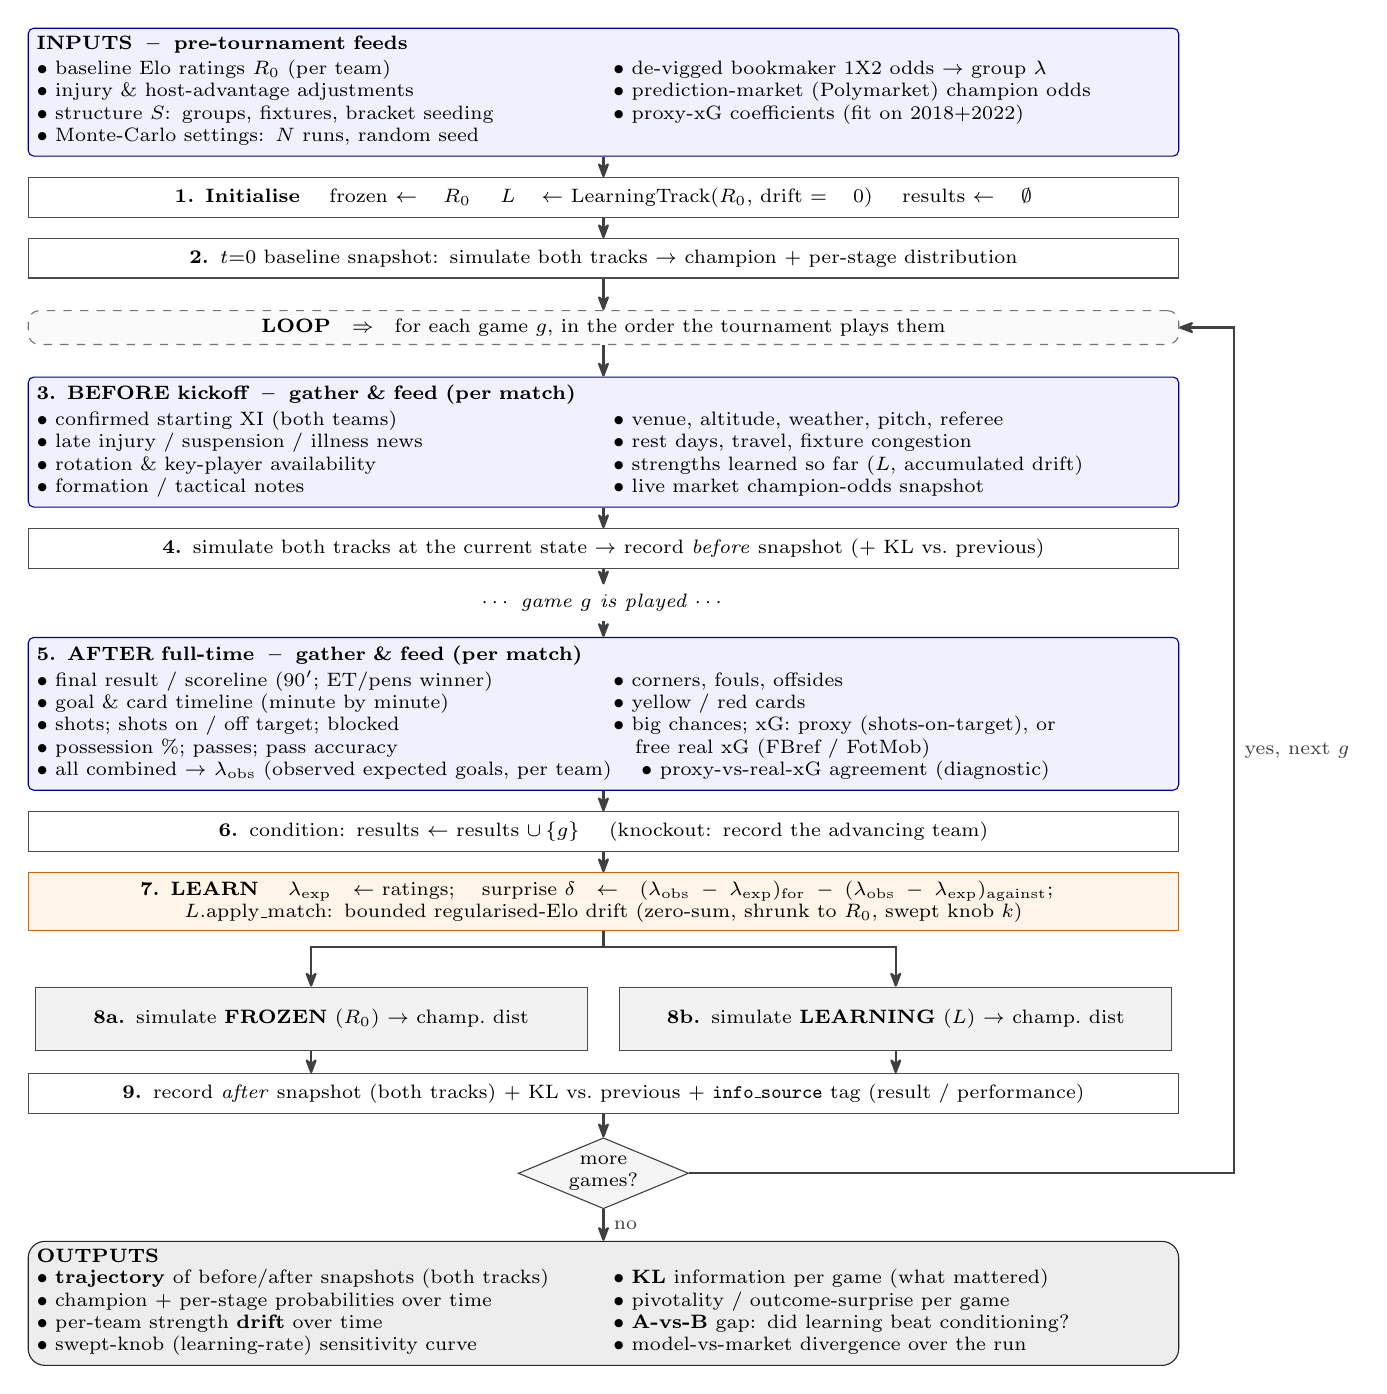
\begin{tikzpicture}[
  font=\scriptsize,
  >={Stealth[round]},
  io/.style={rectangle, rounded corners=2pt, draw=blue!55!black, fill=blue!6, align=left, text width=144mm, inner sep=3pt},
  pbox/.style={rectangle, draw=black!70, fill=white, align=center, text width=144mm, inner sep=3pt, minimum height=5mm},
  learn/.style={rectangle, draw=orange!80!black, fill=orange!9, align=center, text width=144mm, inner sep=3pt},
  sim/.style={rectangle, draw=black!70, fill=black!5, align=center, text width=68mm, inner sep=3pt, minimum height=8mm},
  dec/.style={diamond, draw=black!75, fill=black!4, aspect=2.4, align=center, inner sep=1pt},
  term/.style={rectangle, rounded corners=6pt, draw=black!85, fill=black!7, align=left, text width=144mm, inner sep=3pt},
  a/.style={->, thick, black!75},
  node distance=2.6mm,
]
\node[io] (inp) {\textbf{INPUTS \;\textendash\; pre-tournament feeds}\\[1pt]
\begin{tabular}{@{}p{69mm}p{69mm}@{}}
$\bullet$ baseline Elo ratings $R_0$ (per team) & $\bullet$ de-vigged bookmaker 1X2 odds $\to$ group $\lambda$\\
$\bullet$ injury \& host-advantage adjustments & $\bullet$ prediction-market (Polymarket) champion odds\\
$\bullet$ structure $S$: groups, fixtures, bracket seeding & $\bullet$ proxy-xG coefficients (fit on 2018+2022)\\
$\bullet$ Monte-Carlo settings: $N$ runs, random seed & \\
\end{tabular}};
\node[pbox, below=of inp] (init) {\textbf{1. Initialise} \quad frozen $\leftarrow R_0$ \quad $L \leftarrow$ LearningTrack($R_0$, drift $=0$) \quad results $\leftarrow \emptyset$};
\node[pbox, below=of init] (t0) {\textbf{2.} $t{=}0$ baseline snapshot: simulate both tracks $\rightarrow$ champion $+$ per-stage distribution};
\node[draw=black!55, dashed, fill=black!2, rounded corners, below=4mm of t0, text width=144mm, align=center, inner sep=3pt] (loophead) {\textbf{LOOP} \; $\Rightarrow$ \; for each game $g$, in the order the tournament plays them};
\node[io, below=4mm of loophead] (bef) {\textbf{3. BEFORE kickoff \;\textendash\; gather \& feed (per match)}\\[1pt]
\begin{tabular}{@{}p{69mm}p{69mm}@{}}
$\bullet$ confirmed starting XI (both teams) & $\bullet$ venue, altitude, weather, pitch, referee\\
$\bullet$ late injury / suspension / illness news & $\bullet$ rest days, travel, fixture congestion\\
$\bullet$ rotation \& key-player availability & $\bullet$ strengths learned so far ($L$, accumulated drift)\\
$\bullet$ formation / tactical notes & $\bullet$ live market champion-odds snapshot\\
\end{tabular}};
\node[pbox, below=of bef] (befsim) {\textbf{4.} simulate both tracks at the current state $\rightarrow$ record \emph{before} snapshot ($+$ KL vs.\ previous)};
\node[font=\scriptsize\itshape, below=2mm of befsim] (play) {$\cdots$ game $g$ is played $\cdots$};
\node[io, below=2mm of play] (aft) {\textbf{5. AFTER full-time \;\textendash\; gather \& feed (per match)}\\[1pt]
\begin{tabular}{@{}p{69mm}p{69mm}@{}}
$\bullet$ final result / scoreline (90$'$; ET/pens winner) & $\bullet$ corners, fouls, offsides\\
$\bullet$ goal \& card timeline (minute by minute) & $\bullet$ yellow / red cards\\
$\bullet$ shots; shots on / off target; blocked & $\bullet$ big chances; xG: proxy (shots-on-target), or\\
$\bullet$ possession \%; passes; pass accuracy & \quad free real xG (FBref / FotMob)\\
\multicolumn{2}{@{}l}{$\bullet$ all combined $\rightarrow$ $\lambda_{\text{obs}}$ (observed expected goals, per team) \quad $\bullet$ proxy-vs-real-xG agreement (diagnostic)}\\
\end{tabular}};
\node[pbox, below=of aft] (cond) {\textbf{6.} condition: results $\leftarrow$ results $\cup\,\{g\}$ \quad (knockout: record the advancing team)};
\node[learn, below=of cond] (learn) {\textbf{7. LEARN} \quad $\lambda_{\text{exp}} \leftarrow$ ratings; \;\; surprise $\delta \leftarrow (\lambda_{\text{obs}}-\lambda_{\text{exp}})_{\text{for}} - (\lambda_{\text{obs}}-\lambda_{\text{exp}})_{\text{against}}$; \;\; $L.\text{apply\_match}$: bounded regularised-Elo drift (zero-sum, shrunk to $R_0$, swept knob $k$)};
\node[sim, below left=7mm and 2mm of learn.south] (simf) {\textbf{8a.} simulate \textbf{FROZEN} ($R_0$) $\rightarrow$ champ.\ dist};
\node[sim, below right=7mm and 2mm of learn.south] (siml) {\textbf{8b.} simulate \textbf{LEARNING} ($L$) $\rightarrow$ champ.\ dist};
\node[pbox, below=7mm of learn, yshift=-11mm] (snap) {\textbf{9.} record \emph{after} snapshot (both tracks) $+$ KL vs.\ previous $+$ \texttt{info\_source} tag (result / performance)};
\node[dec, below=3mm of snap] (more) {more\\ games?};
\node[term, below=4mm of more] (out) {\textbf{OUTPUTS}\\[1pt]
\begin{tabular}{@{}p{69mm}p{69mm}@{}}
$\bullet$ \textbf{trajectory} of before/after snapshots (both tracks) & $\bullet$ \textbf{KL} information per game (what mattered)\\
$\bullet$ champion $+$ per-stage probabilities over time & $\bullet$ pivotality / outcome-surprise per game\\
$\bullet$ per-team strength \textbf{drift} over time & $\bullet$ \textbf{A-vs-B} gap: did learning beat conditioning?\\
$\bullet$ swept-knob (learning-rate) sensitivity curve & $\bullet$ model-vs-market divergence over the run\\
\end{tabular}};
% arrows
\draw[a] (inp)--(init);
\draw[a] (init)--(t0);
\draw[a] (t0)--(loophead);
\draw[a] (loophead)--(bef);
\draw[a] (bef)--(befsim);
\draw[a] (befsim)--(play);
\draw[a] (play)--(aft);
\draw[a] (aft)--(cond);
\draw[a] (cond)--(learn);
\draw[a] (learn.south)-- ++(0,-2mm) -| (simf.north);
\draw[a] (learn.south)-- ++(0,-2mm) -| (siml.north);
\draw[a] (simf.south) -- (simf.south|-snap.north);
\draw[a] (siml.south) -- (siml.south|-snap.north);
\draw[a] (snap)--(more);
\draw[a] (more)--(out) node[midway,right,font=\scriptsize]{no};
% loop back on the right
\draw[a] (more.east) -- ([xshift=7mm]bef.east|-more) -- ([xshift=7mm]bef.east|-loophead) node[midway,right,font=\scriptsize]{yes, next $g$} -- (loophead.east);
\end{tikzpicture}
\caption{The two-track living-forecast procedure. A pre-tournament baseline feeds the model; then, for each match, the system gathers and feeds a distinct set of information \emph{before} kickoff (confirmed lineups, late injury and suspension news, and the strengths learned so far) and \emph{after} full-time (the result and the match's performance statistics, converted to an observed expected-goals signal $\lambda_{\text{obs}}$). The frozen track conditions on results with strengths held fixed; the learning track additionally updates each team's strength from $\lambda_{\text{obs}}$ through a regularised-Elo step. Both tracks are re-simulated at every step; the before/after snapshots, the information each carries (KL), and the frozen-versus-learning gap are the outputs.}
\label{fig:algo}
\end{figure}

The information each result carries, again the Kullback--Leibler divergence between the champion distribution before and after it, is concentrated in a few games. The two most informative group matches are Japan's defeats of Germany and Spain, at 0.086 and 0.127 bits against a median group game of 0.026, roughly five times as much, and they are the results that eliminated Germany and reordered Group~E. This repeats on the learning track the uneven-information pattern the frozen backtest of Section~\ref{sec:backtest} already showed.

The learning track sharpens the forecast toward the teams that played well rather than the teams that merely won. At the end of the group stage it rates the two eventual finalists higher than the frozen track does, Argentina at 16.9 against 12.7 percent and France at 18.7 against 14.9 percent, and the two group winners that advanced unconvincingly lower, the Netherlands at 0.9 against 7.9 percent and Spain at 5.9 against 12.6 percent. Argentina's opening defeat to Saudi Arabia shows the mechanism: the result was a 1--2 loss, but Argentina generated 1.95 expected goals to Saudi Arabia's 0.65, so the frozen track reads only the upset while the learning track also reads the dominance, and across the three group games it returns Argentina above its starting strength rather than below it. That same result carried almost no information about the champion's identity (Section~\ref{sec:backtest}), because Argentina still advanced; the performance signal it carried is a separate quantity, and it is the one the learning track is built to use. The estimate suggests that updating on performance, not only on results, moved the 2022 forecast toward the genuinely strong teams, and in this case toward both finalists.

The replay is a sanity check, not a validation, and three things bound it. The baseline ratings are approximate pre-tournament Elo values, the performance signal is a shots-based proxy rather than true expected goals, which is not freely available for the World Cup, and a single tournament cannot separate skill from luck: Brazil, which the learning track rated highest at the end of the group stage at 38.9 against the frozen track's 34.5 percent, went out in the quarter-final on a penalty shootout, an outcome no strength model anticipates. What the replay establishes is that the learning machinery runs end to end on a real tournament and that its adjustments pointed in the direction the eventual results favored. The same two tracks will run live through 2026, where the comparison becomes the pre-registered confirmatory study the framework promises.

\begin{figure}[ht]
\centering

\includegraphics[width=0.95\textwidth]{figs/fig_replay2022.pdf}
\caption{The 2022 World Cup group stage replayed as a living forecast. Top: champion probability for five contenders after each group match, under the learning track (solid, strength updated from performance) and the frozen track (dashed, results only); the learning track raises the eventual finalists Argentina and France and lowers the unconvincing group winners Netherlands and Spain. Bottom: the information each match carries (KL divergence against the previous forecast, in milli-bits), concentrated at Japan's upsets of Germany and Spain.}
\label{fig:replay2022}
\end{figure}

\section{Discussion}

My central design choice is to use market odds where they exist and Elo where they do not, and it follows the empirical finding that betting markets are difficult to beat for match-level football forecasting \citep{strumbelj2014, leitner2010, hvattum2010}. Well-designed hybrid models have outperformed market odds in recent tournaments \citep{groll2019}, so the market tier should be read as a strong baseline rather than an unbeatable one. The slot-emergence criterion itself is not new, because it instantiates the expected-pool-score objective of \citet{kaplangarstka2001}, but the 2026 format gives it unusual bite, because with twelve groups feeding a constrained third-place allocation the gap between head-to-head strength and slot-conditional expected points was large enough to overturn three of 31 knockout entries, two of them robustly (Section~\ref{sec:robust}). Because the group-stage probabilities are recovered from market odds, the entry's edge over a market-literate rival comes entirely from two structural layers, the EV-optimal scoreline selection and the slot-emergence routing.

\subsection{Expected points versus winning the pool}\label{sec:objective}

The optimization target is the entry's own expected points, and this is not identical to the stated goal of winning the pool, which is a rank-order contest against other entrants. The pool literature is explicit about the gap, because when rivals cluster on consensus picks the score-maximizing entry's probability of finishing first can be raised by deviating toward less popular and higher-variance picks \citep{clairletscher2007, kaplangarstka2001}. My entry makes no such deviation, and I did not model the opponents' likely picks.

Two features of the present pool attenuate the gap without closing it. First, the scoring is additive over 104 quasi-independent match calls rather than dominated by a single bracket outcome, so an entry's total concentrates near its expectation and rank order tracks expected points more closely than in winner-take-all bracket pools. Second, the field is small, a friends' pool and not a thousand-entrant office pool, which reduces the duplication pressure that drives contrarian play. If several rivals nonetheless submit near-identical market-consensus entries, the marginal value of my headline picks of Spain and a Spain--Argentina final falls, and a contrarian champion pick could dominate in pool-win probability. Modeling the opponent field, even crudely, is the highest-value extension this framework forgoes.

A second consequence of the objective is how the goal-difference tier governs draws. A draw is rarely the single most probable outcome, but the middle tier rewards a 1--1 prediction on every drawn result, because all draws share goal difference zero, and this makes a draw the expected-value-optimal pick on the most balanced fixtures. The entry therefore predicts a draw on the two most even group games of 2026 and a one-goal favorite on the rest. This already resolves part of the tension between scoring points and resembling reality that a pure exact-score rule would create, because the optimal entry is no longer draw-free, but it does not resolve it fully, since the optimal entry still predicts only a handful of draws against the roughly one-in-four of real matches that end level.

The residual tension can be quantified. An alternative entry that samples each scoreline from its fitted Poisson distribution, rather than taking the optimal pick, reproduces the true draw frequency but gives up points, and backtesting the sampling entry against the optimal entry on 2018 and 2022 measures the cost (Figure~\ref{fig:realism}). The optimal entry scored 67 points in 2018 against the sampling entry's expected 46, a loss of 31 percent, and 48 against 45 in 2022, a loss of 6 percent. The cost of realism is largest exactly when the favorite-based entry does well, in the orderly 2018 tournament, and smallest when favorites disappoint, in the chaotic 2022 tournament, so realism is cheap insurance precisely in the years a points-maximizer least needs it. The three-tier rule pulls the optimal entry partway toward realism on its own, but matching reality fully still costs points.

\begin{figure}[ht]
\centering

\includegraphics[width=\textwidth]{figs/fig_realism.pdf}
\caption{The optimal entry against a realistic, draw-producing alternative that samples each scoreline from its distribution. Left: draws predicted on the 2026 group stage, against the real-tournament average. Right: pool points on the 2018 and 2022 backtests, where the optimal entry scores more in both years, by 31 percent in the orderly 2018 tournament and 6 percent in the upset-heavy 2022 tournament.}
\label{fig:realism}
\end{figure}

\subsection{The Portugal paradox}\label{sec:portugal}

The submitted bracket eliminates Portugal in the Round of 32, and this pick demands explanation, because the market ranks Portugal the sixth-strongest team at outright odds of 10.75 and the simulation gives it an 18.6 percent chance of reaching the semi-finals. The elimination is not a judgment about Portugal's quality. It follows from the way per-match scoring interacts with positional uncertainty, and it is the clearest illustration of criterion~\eqref{eq:slot} at work.

The mechanism has three steps. First, the group forecast places Portugal second in Group K behind Colombia, because the deciding fixture is an Elo near-tie (ratings 1984 against 1977) whose modal outcome favors Colombia by under three percentage points. Second, as Group K runner-up, Portugal is routed to bracket slot M83 against the Group L runner-up, Croatia. Third, and most importantly, Portugal's probability mass is split across two slots, because it wins the group nearly as often as it does not: in the simulation it emerges from the K1 slot (M87) 32.6 percent of the time and from the K2 slot (M83) 25.1 percent of the time. Croatia, by contrast, is concentrated, because England wins Group L in the large majority of simulations, so Croatia lands in M83 with high reliability and emerges from it 27.5 percent of the time. A forecaster who must write one name per slot earns more expected points from the concentrated team than from the stronger but dispersed one (Figure~\ref{fig:slotfig}).

\begin{figure}[ht]
\centering

\includegraphics[width=0.88\textwidth]{figs/fig2_slot_vs_h2h.pdf}
\caption{Head-to-head strength versus slot emergence for the three revised knockout picks. Grey: probability the original pick wins \emph{if the predicted matchup occurs} (Elo). Orange/blue: probability the team actually occupies and wins the bracket slot across 200{,}000 simulations. All three original picks are head-to-head favorites; all three are slot-emergence underdogs.}
\label{fig:slotfig}
\end{figure}

Figure~\ref{fig:slotfig} generalizes the point. In all three revised matches the original pick wins the hypothetical head-to-head, with probabilities between 52.6 and 59.1 percent, and yet it trails in slot emergence. The Turkey case is the extreme, because Turkey is a 55.7 percent head-to-head favorite that reaches its predicted Round-of-16 slot so rarely that its slot emergence is barely above a third of its conditional win probability, and the reason is that its path requires surviving a three-way Group D and then a Round-of-32 tie. What a fixed-bracket forecast can monetize is the concentration of probability mass and not strength.

One caveat qualifies the Portugal call. The pivotal Colombia--Portugal fixture is a matchday-3 game with no published market odds at submission time, so its probabilities rest on the Elo estimate, which is the framework's weakest data tier. If the market had priced Portugal as a clear rather than a marginal favorite in that fixture, Group K would invert and the slot arithmetic would have to be recomputed. Section~\ref{sec:postscript} reports that this is what happened.

\subsection{What can go wrong}

A forecast built for a betting pool should state plainly how it expects to fail. I list six failure modes, ordered roughly by expected damage.

\begin{enumerate}
\item \textbf{The champion call fails (72.6\%).} Spain is the single best pick and still loses most simulated tournaments (Figure~\ref{fig:champdist}). The forecast's defense is that pool points accrue per match: the 72 group scorelines are immune to bracket failure, and they constitute 69\% of scoring opportunities.
\item \textbf{Bracket decay is the norm, not the exception.} The 31 predicted knockout matchups materialize in 2.2--43.9\% of simulations (median 10.4\%). Errors compound multiplicatively down the bracket; the predicted final occurs in 10.8\% of simulations even though it is the most likely one. Late-round predictions are therefore lottery tickets with favorable odds, not expectations.
\item \textbf{A single group upset cascades.} Bracket cells are correlated through the routing graph: if Germany fails to win Group E (it tops the group in roughly half of simulations), at least three knockout entries are invalidated simultaneously. The slot-emergence optimization mitigates but cannot eliminate this correlation.
\item \textbf{Matchday-3 rotation breaks the Elo tier.} A third of group fixtures rest on Elo estimates, concentrated on matchday 3, which is exactly where already-qualified teams rest starters. Elo cannot see rotation, and the market can, but its lines were not yet published at submission. Section~\ref{sec:rotation} identifies this as the model's largest source of error but finds that the status-based correction does not generalize across tournaments; the Colombia--Portugal call (Section~\ref{sec:portugal}) is the highest-stakes exposure.
\item \textbf{Systematic rating error repeats in every simulation.} Monte Carlo dispersion models luck, not miscalibration. Norway (first World Cup since 1998) and several African and Asian sides have thin recent tournament data; the injury adjustments (Brazil $-20$, Netherlands $-15$) are judgment calls with no formal standard error. If any such rating is materially wrong, all 200{,}000 iterations are wrong together.
\item \textbf{Knockout draws resolve as near coin flips.} Around a quarter of knockout matches reach extra time historically; penalty shootouts are close to 50/50 regardless of team strength. The model's Elo-weighted resolution slightly favors stronger sides, overstating their advancement in precisely the matches where strength matters least.
\end{enumerate}

These risks share a common structure, because the model is a point forecast drawn from a distribution it itself estimates to be wide. The pool's per-match scoring works in my favor here, because a strategy of many small and independent calls that are each slightly better than consensus can lose every headline prediction and still win the pool on accumulated group-stage points.

\subsection{Postscript: final pre-kickoff review}\label{sec:postscript}

The pool locks at the June 11 kickoff rather than at the build date, so the forecast incorporates information up to that point through two pre-kickoff revisions. The first is a market recalibration of Group K. On the evening of June 7, before the pool deadline, group-winner prediction markets from Kalshi and Polymarket, in close agreement, became available for the groups whose fixtures lacked match odds. For Group K they priced Portugal at 63 percent and Colombia at 32 percent to win the group, a 2:1 ratio sharply at odds with the Elo near-tie underlying the original forecast, and exactly the contingency I had flagged in Section~\ref{sec:portugal}. Match-level odds remained unpublished, so I incorporated the market signal by calibration, re-deriving the Colombia--Portugal match probabilities from the strength gap of 140 Elo-equivalent points in Portugal's favor at which the simulated group-winner probabilities reproduce the market prices. This yields probabilities of 0.19, 0.24, and 0.57 for the fixture and inverts the predicted group.

The bracket consequences are instructive. I re-simulate with the recalibrated inputs ($N = 50{,}000$), and the results suggest that Portugal's emergence from the K1 slot is 50.7 percent, the strongest slot claim in the entire bracket, so the revised entry sends Portugal past Senegal and Switzerland to a quarter-final exit against Argentina rather than out in the Round of 32. Colombia is now the runner-up and faces Croatia in slot M83, where Croatia's emergence advantage persists at 29.4 against 25.4 percent, so the team that advances from the slot does not change. Every knockout cell's advancing side survives the inversion, and only the group-stage scoreline entry changed. The recalibrated champion distribution moves Portugal from 4.2 to 9.2 percent, close to the 10.8 percent the champion markets themselves price, while Spain (26.9 percent), Argentina (17.9 percent), and France (14.6 percent) are essentially unchanged. The episode is a small validation of the framework's own failure-mode analysis, because the highest-stakes exposure it identified was real, and the repair, once the data arrived, was localized rather than structural.

The second revision is a final injury review in the days before kickoff, after FIFA confirmed the 26-man rosters on June 1 and 2. The most consequential candidate was a hamstring complaint to Argentina's Messi, but the medical reports described muscular fatigue rather than structural damage and the coach confirmed his availability for the opener, so the model's rating of Argentina, the predicted runner-up, was left unchanged; the entry deliberately does not chase the headline. The Netherlands lost the defender Timber to a late withdrawal, which I incorporated as an additional eight-point Elo deduction on top of the deduction already carried for an earlier absence, and the remaining post-roster changes involved squad players rather than starters and were not adjusted. Re-running the simulation with the Timber deduction moves the Netherlands champion probability from 2.6 to 2.4 percent and leaves every other team within Monte Carlo error, and the Netherlands remains the highest-emergence pick in both of its bracket slots, so no entry changes. The final pre-kickoff review therefore confirmed the forecast rather than altering it, which is the outcome a robust entry should produce: the closing injury news was reviewed in full, one small adjustment was made, and the locked predictions stand.

\subsection{How far the model can be improved}\label{sec:audit}

Having located the largest error source in rotation, I tested five further improvements to match-level accuracy on the 2018 and 2022 data, and the audit is as informative for what failed as for what worked (Figure~\ref{fig:audit}). First, in-tournament updating helps. Processing each match in order and updating both teams' Elo by the standard rule with a goal-difference multiplier improves the Brier score of knockout matches by 2.2 percent, because by the knockout stage the ratings have absorbed which teams are actually performing, while the same updating slightly worsens early group-stage prediction, where there is nothing yet to learn. Second, forecast combination did not help on this sample: blending the frozen and the in-tournament-updated forecasts only interpolated between them rather than beating the better one. I read this as an empirical result on two tournaments rather than a general law, because convex combinations of correlated but differently biased forecasts can and often do beat their constituents; here the held-out blend weight simply sat at one of the endpoints. Third, the Dixon--Coles low-score correction \citep{dixoncoles1997} is best judged on the decision rather than the likelihood, since it reshuffles probability among exactly the 0--0, 1--0, 0--1, and 1--1 cells the optimizer selects. Tested that way, it changes 5 of the 72 group picks at the backtest-preferred dependence parameter and raises realized pool points on 2018 and 2022 from 115 to 120, a four percent gain; the parameter is fit in sample, so this is a candidate refinement rather than a validated improvement, but it overturns the earlier likelihood-based claim that the correction does nothing. Independence remains a reasonable default, not a demonstrated optimum.

The fourth test is the most revealing. I obtained each team's expected goals for and against during the 2018 and 2022 tournaments, intending to test an xG-based rating, but this data is in-tournament and using it to predict the same matches would be leakage, so I cannot report a clean predictive gain. What the xG does show, without leakage, is how much of the model's residual error is information and how much is irreducible chance. The teams that dominated on underlying performance frequently went out early: in 2022 Germany had the largest expected-goal difference in the tournament and exited in the group stage, and Brazil had the second largest and lost a quarter-final shootout, while in 2018 Brazil again led on expected goals and fell in the quarter-final. Across both tournaments the correlation between a team's expected-goal difference and the stage it reached is only 0.39, so underlying dominance explains about fifteen percent of how far a team advances and the rest is conversion and chance. The model's largest apparent misses were not failures to identify the strong teams, because the strong teams were correctly identified and simply did not win. This bounds the whole exercise. Match-level prediction can be improved at the margin by learning as the tournament unfolds, but most of what remains unpredictable is not missing information, it is the randomness through which football turns the better performance into the lesser result.

The fifth test puts the sharpest possible case to that conclusion, because it asks whether the archetypal intangible, penalty-shootout temperament, carries any predictive signal. Using the 24 World Cup shootouts from 1998 to 2022, I asked whether the team with the better prior shootout record wins. Only five shootouts involved two teams that each had a prior record and those records differed, and on those five the better-record team won three, a rate indistinguishable from a coin flip. The cumulative records are seductive, with Croatia at four wins and no losses and Argentina at four and one against Spain at one and three and the Netherlands at one and three, and they match the folklore exactly; but they are assembled from the very shootouts one would use them to predict, and prospectively they forecast nothing, because a team contests at most one or two shootouts a tournament and the sample never accumulates. Penalty grit is therefore real as a narrative and absent as a predictor, which is the same lesson the expected-goal analysis gives from the other side: what looks like temperament after the result is, before it, the irreducible coin the tournament tosses.

\begin{figure}[ht]
\centering

\includegraphics[width=\textwidth]{figs/fig_audit.pdf}
\caption{Candidate improvements tested on 2018 and 2022. Left: in-tournament updating improves knockout prediction; forecast combination did not help on this sample; the Dixon--Coles correction, judged on realized points rather than likelihood, gives a small in-sample gain (a fifth test, penalty-shootout temperament, showed no predictive signal and is discussed in the text). Right: expected-goal difference against the stage each team reached, with the correlation only 0.39. The most dominant teams (Brazil, Germany, in red) often went out early, so much of the model's residual error is the irreducible randomness of football rather than missing information.}
\label{fig:audit}
\end{figure}

\subsection{Generalization and the value of information}\label{sec:general}

Two of the paper's results are not specific to football. The slot-emergence rule of Section~\ref{sec:slot} is a statement about a positional loss: when an entry must commit one name to each fixed slot and is scored on whether that slot is filled and won, the optimal pick maximizes a joint probability over occupancy and victory rather than the marginal strength of a team, so the concentrated candidate can beat the stronger but dispersed one. The same argument applies to any fixed-slot prediction contest, from state-by-state electoral-college calls to seeded bracket pools. The information-concentration result is likewise structural: in any sequential-elimination process with a redundant early stage and a winner-take-all back end, most early events are nearly uninformative about the eventual winner and a few late ones are decisive. Primaries before a general election, and the interim looks of a group-sequential clinical trial where most analyses are uninformative and a few are stopping points, share the shape the trajectory traces here.

The connection to decision theory also sharpens what pivotality should measure. The pivotality of Section~\ref{sec:pivotality} is defined on the identity of the champion, which is mutual information, but the objective of this paper is expected pool points, not champion entropy, and the decision-relevant quantity is therefore the value of information \citep{howard1966, raiffa1961}: how much resolving a match changes the optimal entry's expected score. The two can diverge, because a group result can be pivotal for pool points by invalidating several knockout slot picks while moving the champion distribution by almost nothing. Appendix~\ref{app:survival} already estimates this score-metric pivotality through the surrogate sensitivity analysis, which asks which group calls most affect the entry's downstream knockout score, and a fuller treatment would compute the value of information directly on the score rather than on the champion. I flag this as the most promising extension, because it would replace a champion-entropy instrument with one matched to the actual decision.

\subsection{Limitations}

The historical backtest of Section~\ref{sec:backtest} validates calibration on 2018 and 2022, but it tests the Elo-based pipeline rather than the market-calibrated group stage of 2026, and it cannot exercise the slot-emergence routing, which the 32-team format of those tournaments does not contain. The framework's full empirical standing therefore still rests on the forthcoming out-of-sample evaluation against the realized 2026 tournament, for which all predictions are timestamped and locked. Team strength is also frozen at the June 11 pre-kickoff lock, reviewed against the final squad and injury news as described in Section~\ref{sec:postscript}, because the pool's all-entries-before-kickoff rule makes within-tournament resubmission impossible, though Section~\ref{sec:audit} shows that within-tournament updating would improve a forecast not bound by that rule. The goal model assumes independent Poisson margins; Section~\ref{sec:audit} shows that a Dixon--Coles dependence correction changes a few picks and gives a small in-sample points gain, so independence is a reasonable default rather than a demonstrated optimum, and a fitted dependence parameter is a candidate refinement for future entries.

Post-tournament, the forecast will be evaluated against realized results match by match; the prediction sheet includes tracking columns for this purpose.

\section*{Declarations}

\noindent\textbf{Data availability.} All input data (odds snapshots, Elo ratings, squad news), model code (Poisson fitting, knockout model, tournament simulator, sensitivity sweep), and the generated prediction sheet are available from the author. Reproducibility parameters: Poisson rates fitted by grid search with step 0.05 over $\lambda \in [0.10, 3.50]$; simulations use $N = 200{,}000$ iterations with fixed seed 2026 (sensitivity sweep: $N = 20{,}000$ per configuration, same seed).

\noindent\textbf{Ethics.} The forecast supports a private, small-stakes prediction pool among friends; no commercial betting activity is involved.

\noindent\textbf{Author contributions (CRediT).} Avralt-Od Purevjav: conceptualization, methodology, software, formal analysis, writing.

\noindent\textbf{Conflict of interest.} The author intends to win the pool.

\noindent\textbf{Funding.} None.

\noindent\textbf{AI disclosure.} Model design, data collection, simulation code, and manuscript drafting were carried out with the assistance of Claude (Anthropic); all modeling decisions and the final predictions were reviewed and approved by the author.

\appendix

\section{Group-stage forecast rationale}\label{app:groups}

Predicted finishing order per group, with the decisive evidence. Advancers are the top two plus the eight best third-placed teams; the model's third-place qualifiers are Senegal and Ivory Coast (goal difference 0) and Paraguay, Sweden, Bosnia and Herzegovina, Algeria, Iran, and Czechia (all $-1$); Scotland, Cape Verde, Uzbekistan ($-2$) and Ghana ($-3$) miss the cut.

Figure~\ref{fig:groupqual} shows each team's qualification probability from 100{,}000 simulations, decomposed into winning the group, finishing second, and advancing as a best third-placed team. Table~\ref{tab:qual} reports the same probabilities numerically. The competitiveness of the twelve groups varies widely. Group A is the tightest, because Czechia and South Korea finish within two percentage points of each other for the second qualification place, while Groups K and L are the most decided, because two strong teams in each take roughly 95 percent of the qualification mass between them and leave the other two with little.

\begin{figure}[p]
\centering

\includegraphics[width=0.96\textwidth]{figs/fig_group_qual.pdf}
\caption{Qualification probability by team across 100{,}000 simulations. Dark blue is the probability of winning the group, light blue of finishing second, orange of advancing as one of the eight best third-placed teams, and grey of elimination. The number at each bar is the total qualification probability.}
\label{fig:groupqual}
\end{figure}

\begin{table}[ht]
\centering\scriptsize
\caption{Qualification probabilities by team (percent), 100{,}000 simulations. Columns report the probability of winning the group, finishing second, advancing as a best third-placed team ($^{*}$), and qualifying in total.}
\label{tab:qual}
\begin{minipage}{0.49\textwidth}\centering
\begin{tabular}{llcccc}
\toprule
Grp & Team & 1st & 2nd & 3rd$^{*}$ & Qual \\
\midrule
A & Mexico & 55 & 26 & 11 & \textbf{91} \\
 & Czechia & 19 & 29 & 20 & \textbf{68} \\
 & South Korea & 18 & 28 & 21 & \textbf{66} \\
 & South Africa & 8 & 18 & 19 & \textbf{45} \\
\addlinespace
B & Switzerland & 54 & 29 & 10 & \textbf{94} \\
 & Canada & 33 & 38 & 17 & \textbf{88} \\
 & Bosnia and He. & 10 & 24 & 28 & \textbf{62} \\
 & Qatar & 2 & 8 & 13 & \textbf{24} \\
\addlinespace
C & Brazil & 68 & 23 & 7 & \textbf{98} \\
 & Morocco & 22 & 46 & 20 & \textbf{89} \\
 & Scotland & 10 & 27 & 33 & \textbf{69} \\
 & Haiti & 0 & 4 & 8 & \textbf{12} \\
\addlinespace
D & United States & 37 & 29 & 16 & \textbf{82} \\
 & Turkey & 35 & 29 & 17 & \textbf{81} \\
 & Paraguay & 18 & 25 & 22 & \textbf{65} \\
 & Australia & 10 & 17 & 18 & \textbf{45} \\
\addlinespace
E & Germany & 67 & 24 & 8 & \textbf{99} \\
 & Ecuador & 20 & 42 & 26 & \textbf{88} \\
 & Ivory Coast & 13 & 33 & 36 & \textbf{82} \\
 & Curaçao & 0 & 2 & 5 & \textbf{7} \\
\addlinespace
F & Netherlands & 53 & 26 & 12 & \textbf{91} \\
 & Japan & 25 & 32 & 19 & \textbf{76} \\
 & Sweden & 15 & 26 & 22 & \textbf{64} \\
 & Tunisia & 7 & 16 & 18 & \textbf{40} \\
\addlinespace
\bottomrule
\end{tabular}
\end{minipage}\hfill
\begin{minipage}{0.49\textwidth}\centering
\begin{tabular}{llcccc}
\toprule
Grp & Team & 1st & 2nd & 3rd$^{*}$ & Qual \\
\midrule
G & Belgium & 68 & 21 & 7 & \textbf{96} \\
 & Egypt & 18 & 38 & 20 & \textbf{76} \\
 & Iran & 10 & 28 & 24 & \textbf{63} \\
 & New Zealand & 3 & 12 & 15 & \textbf{31} \\
\addlinespace
H & Spain & 75 & 21 & 3 & \textbf{99} \\
 & Uruguay & 21 & 54 & 13 & \textbf{88} \\
 & Cape Verde & 2 & 12 & 20 & \textbf{35} \\
 & Saudi Arabia & 2 & 13 & 19 & \textbf{34} \\
\addlinespace
I & France & 62 & 26 & 10 & \textbf{98} \\
 & Norway & 24 & 41 & 25 & \textbf{90} \\
 & Senegal & 13 & 31 & 38 & \textbf{82} \\
 & Iraq & 0 & 2 & 5 & \textbf{8} \\
\addlinespace
J & Argentina & 82 & 14 & 3 & \textbf{99} \\
 & Austria & 10 & 45 & 21 & \textbf{76} \\
 & Algeria & 7 & 29 & 22 & \textbf{57} \\
 & Jordan & 2 & 12 & 15 & \textbf{29} \\
\addlinespace
K & Portugal & 63 & 28 & 6 & \textbf{97} \\
 & Colombia & 32 & 51 & 11 & \textbf{94} \\
 & Uzbekistan & 3 & 12 & 23 & \textbf{39} \\
 & Congo DR & 2 & 8 & 18 & \textbf{29} \\
\addlinespace
L & England & 68 & 27 & 4 & \textbf{99} \\
 & Croatia & 29 & 56 & 10 & \textbf{96} \\
 & Panama & 3 & 12 & 21 & \textbf{36} \\
 & Ghana & 0 & 4 & 18 & \textbf{23} \\
\addlinespace
\bottomrule
\end{tabular}
\end{minipage}
\end{table}

\begin{table}[ht]
\centering\small
\caption{Decisive fixture and primary forecast risk by group. The decisive fixture is the match that, in the simulations, most often determines the second qualification place; the primary risk is the most probable way the submitted group order is wrong.}
\label{tab:watchrisk}
\begin{tabular}{p{0.5cm}p{5.4cm}p{6.6cm}}
\toprule
Grp & Decisive fixture & Primary risk to the forecast \\
\midrule
A & South Korea vs.\ Czechia, matchday 1 & Czechia (68\% qual.) takes second ahead of South Korea \\
B & Switzerland vs.\ Canada, matchday 3 & Host Canada (88\%) wins the group outright \\
C & Scotland vs.\ Morocco, matchday 2 & Scotland (69\%) overtakes Morocco for second \\
D & Turkey vs.\ United States, matchday 3 & Turkey tops the group and reroutes the bracket \\
E & Ecuador vs.\ Germany, matchday 3 & Ecuador (88\%, Elo 1935) wins the group, not second \\
F & Netherlands vs.\ Japan, matchday 1 & Japan (76\%) wins the group ahead of the Netherlands \\
G & Egypt vs.\ Iran, matchday 3 & Iran (63\%) edges Egypt for second \\
H & Cape Verde vs.\ Saudi Arabia (third-place race) & Neither third-placer qualifies; Uruguay slips to second \\
I & Norway vs.\ Senegal, matchday 2 & Senegal (82\%) beats Norway and takes second \\
J & Algeria vs.\ Austria, matchday 3 & Algeria (57\%) overtakes Austria for second \\
K & Colombia vs.\ Portugal, matchday 3 & The Elo tie holds and Colombia (94\%) tops the group \\
L & England vs.\ Croatia, matchday 1 & Croatia (96\%) wins the group instead of England \\
\bottomrule
\end{tabular}
\end{table}

The group-by-group rationale follows; each paragraph states the decisive evidence behind the predicted order.

\paragraph{Group A (Mexico, South Korea, Czechia, South Africa).} Mexico tops the group on the tournament's clearest host signal, because the opener is at Estadio Azteca at 2{,}240 m altitude, the market prices Mexico at 68 percent, and the striker is in form. Second place is the group's only genuine toss-up, and South Korea over Czechia rests on a 23-point Elo edge of 1756 against 1733, so their direct meeting on matchday 1 effectively decides the order. Czechia advances third.

\noindent\textit{\footnotesize Predicted group table (each cell: row team's score against the column team, then the prediction's expected points in parentheses; G = goal difference, P = points):}

\noindent{\footnotesize\begin{tabular}{@{}clcccccccr@{}}
\toprule
 & Team & \resizebox{4mm}{2.7mm}{\worldflag[width=10mm]{MX}} & \resizebox{4mm}{2.7mm}{\worldflag[width=10mm]{KR}} & \resizebox{4mm}{2.7mm}{\worldflag[width=10mm]{CZ}} & \resizebox{4mm}{2.7mm}{\worldflag[width=10mm]{ZA}} & W & L & G & P \\
\midrule
1 & \resizebox{4mm}{2.7mm}{\worldflag[width=10mm]{MX}}~\textbf{Mexico} & --- & 1--0\,{\scriptsize(0.95)} & 1--0\,{\scriptsize(0.90)} & 1--0\,{\scriptsize(1.08)} & 3 & 0 & $+$3 & \textbf{9} \\
2 & \resizebox{4mm}{2.7mm}{\worldflag[width=10mm]{KR}}~\textbf{South Korea} & 0--1\,{\scriptsize(0.95)} & --- & 1--1\,{\scriptsize(0.74)} & 1--0\,{\scriptsize(0.79)} & 1 & 1 & 0 & \textbf{4} \\
3 & \resizebox{4mm}{2.7mm}{\worldflag[width=10mm]{CZ}}~Czechia & 0--1\,{\scriptsize(0.90)} & 1--1\,{\scriptsize(0.74)} & --- & 1--0\,{\scriptsize(0.84)} & 1 & 1 & 0 & 4 \\
4 & \resizebox{4mm}{2.7mm}{\worldflag[width=10mm]{ZA}}~South Africa & 0--1\,{\scriptsize(1.08)} & 0--1\,{\scriptsize(0.79)} & 0--1\,{\scriptsize(0.84)} & --- & 0 & 3 & -3 & 0 \\
\bottomrule
\end{tabular}}


\paragraph{Group B (Switzerland, Canada, Bosnia and Herzegovina, Qatar).} Switzerland carries the group's highest rating (Elo 1894) and a 50\% vs.\ 30\% market edge in the decider against host Canada. Qatar is the weakest side in the field (Elo 1423), making goal difference against them the implicit tiebreaker currency. Bosnia advances third via the Qatar fixture.

\noindent\textit{\footnotesize Predicted group table (each cell: row team's score against the column team, then the prediction's expected points in parentheses; G = goal difference, P = points):}

\noindent{\footnotesize\begin{tabular}{@{}clcccccccr@{}}
\toprule
 & Team & \resizebox{4mm}{2.7mm}{\worldflag[width=10mm]{CH}} & \resizebox{4mm}{2.7mm}{\worldflag[width=10mm]{CA}} & \resizebox{4mm}{2.7mm}{\worldflag[width=10mm]{BA}} & \resizebox{4mm}{2.7mm}{\worldflag[width=10mm]{QA}} & W & L & G & P \\
\midrule
1 & \resizebox{4mm}{2.7mm}{\worldflag[width=10mm]{CH}}~\textbf{Switzerland} & --- & 2--1\,{\scriptsize(0.80)} & 1--0\,{\scriptsize(1.03)} & 1--0\,{\scriptsize(1.08)} & 3 & 0 & $+$3 & \textbf{9} \\
2 & \resizebox{4mm}{2.7mm}{\worldflag[width=10mm]{CA}}~\textbf{Canada} & 1--2\,{\scriptsize(0.80)} & --- & 1--0\,{\scriptsize(0.90)} & 1--0\,{\scriptsize(1.12)} & 2 & 1 & $+$1 & \textbf{6} \\
3 & \resizebox{4mm}{2.7mm}{\worldflag[width=10mm]{BA}}~Bosnia and Herzegovina & 0--1\,{\scriptsize(1.03)} & 0--1\,{\scriptsize(0.90)} & --- & 1--0\,{\scriptsize(0.95)} & 1 & 2 & -1 & 3 \\
4 & \resizebox{4mm}{2.7mm}{\worldflag[width=10mm]{QA}}~Qatar & 0--1\,{\scriptsize(1.08)} & 0--1\,{\scriptsize(1.12)} & 0--1\,{\scriptsize(0.95)} & --- & 0 & 3 & -3 & 0 \\
\bottomrule
\end{tabular}}


\paragraph{Group C (Brazil, Morocco, Scotland, Haiti).} Brazil wins the group despite the Rodrygo injury (rating adjusted $-20$); an Elo of 1988 and an 87\% market price against Haiti absorb the loss. The pivotal fixture is Scotland--Morocco for second, where the market is unambiguous (50\% vs.\ 23\% for Morocco). Scotland's three points are eliminated on goal difference.

\noindent\textit{\footnotesize Predicted group table (each cell: row team's score against the column team, then the prediction's expected points in parentheses; G = goal difference, P = points):}

\noindent{\footnotesize\begin{tabular}{@{}clcccccccr@{}}
\toprule
 & Team & \resizebox{4mm}{2.7mm}{\worldflag[width=10mm]{BR}} & \resizebox{4mm}{2.7mm}{\worldflag[width=10mm]{MA}} & \resizebox{4mm}{2.7mm}{\flagSCO[10mm]} & \resizebox{4mm}{2.7mm}{\worldflag[width=10mm]{HT}} & W & L & G & P \\
\midrule
1 & \resizebox{4mm}{2.7mm}{\worldflag[width=10mm]{BR}}~\textbf{Brazil} & --- & 1--0\,{\scriptsize(0.97)} & 1--0\,{\scriptsize(1.05)} & 2--0\,{\scriptsize(1.37)} & 3 & 0 & $+$4 & \textbf{9} \\
2 & \resizebox{4mm}{2.7mm}{\worldflag[width=10mm]{MA}}~\textbf{Morocco} & 0--1\,{\scriptsize(0.97)} & --- & 1--0\,{\scriptsize(0.90)} & 1--0\,{\scriptsize(1.28)} & 2 & 1 & $+$1 & \textbf{6} \\
3 & \resizebox{4mm}{2.7mm}{\flagSCO[10mm]}~Scotland & 0--1\,{\scriptsize(1.05)} & 0--1\,{\scriptsize(0.90)} & --- & 1--0\,{\scriptsize(1.00)} & 1 & 2 & -1 & 3 \\
4 & \resizebox{4mm}{2.7mm}{\worldflag[width=10mm]{HT}}~Haiti & 0--2\,{\scriptsize(1.37)} & 0--1\,{\scriptsize(1.28)} & 0--1\,{\scriptsize(1.00)} & --- & 0 & 3 & -4 & 0 \\
\bottomrule
\end{tabular}}


\paragraph{Group D (United States, Turkey, Paraguay, Australia).} The tightest group in the tournament and the bracket's largest group-stage risk. Turkey holds the higher rating (Elo 1906), but the United States carries the host adjustment and the group-winner market (40\% vs.\ 35\%). The head-to-head was priced at an exact tie (36.3\%/36.3\%); the submitted scoreline is the expected-value-optimal 1--1 draw, and the entry assigns the group-winner slot to the United States because simulation showed that routing places both teams in bracket slots they survive more often (Section 4.2). Paraguay advances third.

\noindent\textit{\footnotesize Predicted group table (each cell: row team's score against the column team, then the prediction's expected points in parentheses; G = goal difference, P = points):}

\noindent{\footnotesize\begin{tabular}{@{}clcccccccr@{}}
\toprule
 & Team & \resizebox{4mm}{2.7mm}{\worldflag[width=10mm]{US}} & \resizebox{4mm}{2.7mm}{\worldflag[width=10mm]{TR}} & \resizebox{4mm}{2.7mm}{\worldflag[width=10mm]{PY}} & \resizebox{4mm}{2.7mm}{\worldflag[width=10mm]{AU}} & W & L & G & P \\
\midrule
1 & \resizebox{4mm}{2.7mm}{\worldflag[width=10mm]{US}}~\textbf{United States} & --- & 1--1\,{\scriptsize(0.68)} & 1--0\,{\scriptsize(0.86)} & 1--0\,{\scriptsize(0.95)} & 2 & 0 & $+$2 & \textbf{7} \\
2 & \resizebox{4mm}{2.7mm}{\worldflag[width=10mm]{TR}}~\textbf{Turkey} & 1--1\,{\scriptsize(0.68)} & --- & 1--0\,{\scriptsize(0.82)} & 1--0\,{\scriptsize(0.94)} & 2 & 0 & $+$2 & \textbf{7} \\
3 & \resizebox{4mm}{2.7mm}{\worldflag[width=10mm]{PY}}~Paraguay & 0--1\,{\scriptsize(0.86)} & 0--1\,{\scriptsize(0.82)} & --- & 1--0\,{\scriptsize(0.85)} & 1 & 2 & -1 & 3 \\
4 & \resizebox{4mm}{2.7mm}{\worldflag[width=10mm]{AU}}~Australia & 0--1\,{\scriptsize(0.95)} & 0--1\,{\scriptsize(0.94)} & 0--1\,{\scriptsize(0.85)} & --- & 0 & 3 & -3 & 0 \\
\bottomrule
\end{tabular}}


\paragraph{Group E (Germany, Ecuador, Ivory Coast, Curaçao).} Germany--Curaçao is the tournament's heaviest mismatch at 92 percent, and it produces the forecast's only 3--0. Ecuador's rating of Elo 1935 exceeds several traditional powers', and the 42 against 28 percent market edge over Ivory Coast settles second. Ivory Coast advances as one of the two strongest third-placers.

\noindent\textit{\footnotesize Predicted group table (each cell: row team's score against the column team, then the prediction's expected points in parentheses; G = goal difference, P = points):}

\noindent{\footnotesize\begin{tabular}{@{}clcccccccr@{}}
\toprule
 & Team & \resizebox{4mm}{2.7mm}{\worldflag[width=10mm]{DE}} & \resizebox{4mm}{2.7mm}{\worldflag[width=10mm]{EC}} & \resizebox{4mm}{2.7mm}{\worldflag[width=10mm]{CI}} & \resizebox{4mm}{2.7mm}{\flagCUW[10mm]} & W & L & G & P \\
\midrule
1 & \resizebox{4mm}{2.7mm}{\worldflag[width=10mm]{DE}}~\textbf{Germany} & --- & 1--0\,{\scriptsize(0.95)} & 1--0\,{\scriptsize(1.04)} & 3--0\,{\scriptsize(1.32)} & 3 & 0 & $+$5 & \textbf{9} \\
2 & \resizebox{4mm}{2.7mm}{\worldflag[width=10mm]{EC}}~\textbf{Ecuador} & 0--1\,{\scriptsize(0.95)} & --- & 1--0\,{\scriptsize(0.83)} & 2--0\,{\scriptsize(1.15)} & 2 & 1 & $+$2 & \textbf{6} \\
3 & \resizebox{4mm}{2.7mm}{\worldflag[width=10mm]{CI}}~Ivory Coast & 0--1\,{\scriptsize(1.04)} & 0--1\,{\scriptsize(0.83)} & --- & 2--0\,{\scriptsize(1.15)} & 1 & 2 & 0 & 3 \\
4 & \resizebox{4mm}{2.7mm}{\flagCUW[10mm]}~Curaçao & 0--3\,{\scriptsize(1.32)} & 0--2\,{\scriptsize(1.15)} & 0--2\,{\scriptsize(1.15)} & --- & 0 & 3 & -7 & 0 \\
\bottomrule
\end{tabular}}


\paragraph{Group F (Netherlands, Japan, Sweden, Tunisia).} The opening Netherlands--Japan fixture effectively decides the group (46\% vs.\ 28\%). The Dutch absorb the Xavi Simons loss ($-15$); Japan's Mitoma absence ($-10$) trims a key attacking channel but leaves second place secure. Sweden advances third on the Tunisia result.

\noindent\textit{\footnotesize Predicted group table (each cell: row team's score against the column team, then the prediction's expected points in parentheses; G = goal difference, P = points):}

\noindent{\footnotesize\begin{tabular}{@{}clcccccccr@{}}
\toprule
 & Team & \resizebox{4mm}{2.7mm}{\worldflag[width=10mm]{NL}} & \resizebox{4mm}{2.7mm}{\worldflag[width=10mm]{JP}} & \resizebox{4mm}{2.7mm}{\worldflag[width=10mm]{SE}} & \resizebox{4mm}{2.7mm}{\worldflag[width=10mm]{TN}} & W & L & G & P \\
\midrule
1 & \resizebox{4mm}{2.7mm}{\worldflag[width=10mm]{NL}}~\textbf{Netherlands} & --- & 1--0\,{\scriptsize(0.81)} & 1--0\,{\scriptsize(0.99)} & 1--0\,{\scriptsize(1.04)} & 3 & 0 & $+$3 & \textbf{9} \\
2 & \resizebox{4mm}{2.7mm}{\worldflag[width=10mm]{JP}}~\textbf{Japan} & 0--1\,{\scriptsize(0.81)} & --- & 1--0\,{\scriptsize(0.77)} & 1--0\,{\scriptsize(0.94)} & 2 & 1 & $+$1 & \textbf{6} \\
3 & \resizebox{4mm}{2.7mm}{\worldflag[width=10mm]{SE}}~Sweden & 0--1\,{\scriptsize(0.99)} & 0--1\,{\scriptsize(0.77)} & --- & 1--0\,{\scriptsize(0.89)} & 1 & 2 & -1 & 3 \\
4 & \resizebox{4mm}{2.7mm}{\worldflag[width=10mm]{TN}}~Tunisia & 0--1\,{\scriptsize(1.04)} & 0--1\,{\scriptsize(0.94)} & 0--1\,{\scriptsize(0.89)} & --- & 0 & 3 & -3 & 0 \\
\bottomrule
\end{tabular}}


\paragraph{Group G (Belgium, Egypt, Iran, New Zealand).} This is the weakest group by aggregate rating. Belgium wins it at modest strength, and this matters later, because the soft path inflates Belgium's slot emergence in the knockout phase (Section 4.2). Egypt over Iran decides second at 42 against 27 percent, and Iran advances third.

\noindent\textit{\footnotesize Predicted group table (each cell: row team's score against the column team, then the prediction's expected points in parentheses; G = goal difference, P = points):}

\noindent{\footnotesize\begin{tabular}{@{}clcccccccr@{}}
\toprule
 & Team & \resizebox{4mm}{2.7mm}{\worldflag[width=10mm]{BE}} & \resizebox{4mm}{2.7mm}{\worldflag[width=10mm]{EG}} & \resizebox{4mm}{2.7mm}{\worldflag[width=10mm]{IR}} & \resizebox{4mm}{2.7mm}{\worldflag[width=10mm]{NZ}} & W & L & G & P \\
\midrule
1 & \resizebox{4mm}{2.7mm}{\worldflag[width=10mm]{BE}}~\textbf{Belgium} & --- & 1--0\,{\scriptsize(0.96)} & 1--0\,{\scriptsize(1.06)} & 2--0\,{\scriptsize(1.12)} & 3 & 0 & $+$4 & \textbf{9} \\
2 & \resizebox{4mm}{2.7mm}{\worldflag[width=10mm]{EG}}~\textbf{Egypt} & 0--1\,{\scriptsize(0.96)} & --- & 1--0\,{\scriptsize(0.83)} & 1--0\,{\scriptsize(1.00)} & 2 & 1 & $+$1 & \textbf{6} \\
3 & \resizebox{4mm}{2.7mm}{\worldflag[width=10mm]{IR}}~Iran & 0--1\,{\scriptsize(1.06)} & 0--1\,{\scriptsize(0.83)} & --- & 1--0\,{\scriptsize(0.91)} & 1 & 2 & -1 & 3 \\
4 & \resizebox{4mm}{2.7mm}{\worldflag[width=10mm]{NZ}}~New Zealand & 0--2\,{\scriptsize(1.12)} & 0--1\,{\scriptsize(1.00)} & 0--1\,{\scriptsize(0.91)} & --- & 0 & 3 & -4 & 0 \\
\bottomrule
\end{tabular}}


\paragraph{Group H (Spain, Uruguay, Cape Verde, Saudi Arabia).} The champion pick's runway: Spain is the field's highest-rated team (Elo 2165) and an 85\%+ market favorite in two of three fixtures. Uruguay's healthy squad takes second. Cape Verde's three points fall on goal difference.

\noindent\textit{\footnotesize Predicted group table (each cell: row team's score against the column team, then the prediction's expected points in parentheses; G = goal difference, P = points):}

\noindent{\footnotesize\begin{tabular}{@{}clcccccccr@{}}
\toprule
 & Team & \resizebox{4mm}{2.7mm}{\worldflag[width=10mm]{ES}} & \resizebox{4mm}{2.7mm}{\worldflag[width=10mm]{UY}} & \resizebox{4mm}{2.7mm}{\worldflag[width=10mm]{CV}} & \resizebox{4mm}{2.7mm}{\worldflag[width=10mm]{SA}} & W & L & G & P \\
\midrule
1 & \resizebox{4mm}{2.7mm}{\worldflag[width=10mm]{ES}}~\textbf{Spain} & --- & 1--0\,{\scriptsize(0.98)} & 2--0\,{\scriptsize(1.22)} & 2--0\,{\scriptsize(1.18)} & 3 & 0 & $+$5 & \textbf{9} \\
2 & \resizebox{4mm}{2.7mm}{\worldflag[width=10mm]{UY}}~\textbf{Uruguay} & 0--1\,{\scriptsize(0.98)} & --- & 1--0\,{\scriptsize(1.08)} & 1--0\,{\scriptsize(1.02)} & 2 & 1 & $+$1 & \textbf{6} \\
3 & \resizebox{4mm}{2.7mm}{\worldflag[width=10mm]{CV}}~Cape Verde & 0--2\,{\scriptsize(1.22)} & 0--1\,{\scriptsize(1.08)} & --- & 1--0\,{\scriptsize(0.75)} & 1 & 2 & -2 & 3 \\
4 & \resizebox{4mm}{2.7mm}{\worldflag[width=10mm]{SA}}~Saudi Arabia & 0--2\,{\scriptsize(1.18)} & 0--1\,{\scriptsize(1.02)} & 0--1\,{\scriptsize(0.75)} & --- & 0 & 3 & -4 & 0 \\
\bottomrule
\end{tabular}}


\paragraph{Group I (France, Norway, Senegal, Iraq).} France tops the group at a 66 percent market price. Norway is at a first World Cup since 1998 and the group-winner market puts it at 24 percent against Senegal's 10 percent, so Norway takes second via the matchday-2 meeting with Senegal (Elo 1917 against 1866). Senegal advances as the tournament's strongest third-placer, which is consequential, because it is the predicted Round-of-32 opponent in Portugal's slot.

\noindent\textit{\footnotesize Predicted group table (each cell: row team's score against the column team, then the prediction's expected points in parentheses; G = goal difference, P = points):}

\noindent{\footnotesize\begin{tabular}{@{}clcccccccr@{}}
\toprule
 & Team & \resizebox{4mm}{2.7mm}{\worldflag[width=10mm]{FR}} & \resizebox{4mm}{2.7mm}{\worldflag[width=10mm]{NO}} & \resizebox{4mm}{2.7mm}{\worldflag[width=10mm]{SN}} & \resizebox{4mm}{2.7mm}{\worldflag[width=10mm]{IQ}} & W & L & G & P \\
\midrule
1 & \resizebox{4mm}{2.7mm}{\worldflag[width=10mm]{FR}}~\textbf{France} & --- & 1--0\,{\scriptsize(0.94)} & 1--0\,{\scriptsize(1.02)} & 2--0\,{\scriptsize(1.35)} & 3 & 0 & $+$4 & \textbf{9} \\
2 & \resizebox{4mm}{2.7mm}{\worldflag[width=10mm]{NO}}~\textbf{Norway} & 0--1\,{\scriptsize(0.94)} & --- & 1--0\,{\scriptsize(0.88)} & 2--0\,{\scriptsize(1.12)} & 2 & 1 & $+$2 & \textbf{6} \\
3 & \resizebox{4mm}{2.7mm}{\worldflag[width=10mm]{SN}}~Senegal & 0--1\,{\scriptsize(1.02)} & 0--1\,{\scriptsize(0.88)} & --- & 2--0\,{\scriptsize(1.11)} & 1 & 2 & 0 & 3 \\
4 & \resizebox{4mm}{2.7mm}{\worldflag[width=10mm]{IQ}}~Iraq & 0--2\,{\scriptsize(1.35)} & 0--2\,{\scriptsize(1.12)} & 0--2\,{\scriptsize(1.11)} & --- & 0 & 3 & -6 & 0 \\
\bottomrule
\end{tabular}}


\paragraph{Group J (Argentina, Austria, Algeria, Jordan).} The lowest-variance group for the bracket: Argentina (Elo 2113) is a 63\%+ favorite in every fixture. Austria (Elo 1830) beats Algeria in the decider for second (43\% vs.\ 28\%); Algeria advances third.

\noindent\textit{\footnotesize Predicted group table (each cell: row team's score against the column team, then the prediction's expected points in parentheses; G = goal difference, P = points):}

\noindent{\footnotesize\begin{tabular}{@{}clcccccccr@{}}
\toprule
 & Team & \resizebox{4mm}{2.7mm}{\worldflag[width=10mm]{AR}} & \resizebox{4mm}{2.7mm}{\worldflag[width=10mm]{AT}} & \resizebox{4mm}{2.7mm}{\worldflag[width=10mm]{DZ}} & \resizebox{4mm}{2.7mm}{\worldflag[width=10mm]{JO}} & W & L & G & P \\
\midrule
1 & \resizebox{4mm}{2.7mm}{\worldflag[width=10mm]{AR}}~\textbf{Argentina} & --- & 2--0\,{\scriptsize(1.15)} & 1--0\,{\scriptsize(1.08)} & 2--0\,{\scriptsize(1.22)} & 3 & 0 & $+$5 & \textbf{9} \\
2 & \resizebox{4mm}{2.7mm}{\worldflag[width=10mm]{AT}}~\textbf{Austria} & 0--2\,{\scriptsize(1.15)} & --- & 1--0\,{\scriptsize(0.80)} & 1--0\,{\scriptsize(1.07)} & 2 & 1 & 0 & \textbf{6} \\
3 & \resizebox{4mm}{2.7mm}{\worldflag[width=10mm]{DZ}}~Algeria & 0--1\,{\scriptsize(1.08)} & 0--1\,{\scriptsize(0.80)} & --- & 1--0\,{\scriptsize(0.75)} & 1 & 2 & -1 & 3 \\
4 & \resizebox{4mm}{2.7mm}{\worldflag[width=10mm]{JO}}~Jordan & 0--2\,{\scriptsize(1.22)} & 0--1\,{\scriptsize(1.07)} & 0--1\,{\scriptsize(0.75)} & --- & 0 & 3 & -4 & 0 \\
\bottomrule
\end{tabular}}


\paragraph{Group K (Portugal, Colombia, Uzbekistan, Congo DR).} This is the recalibrated group (Section 5.4). Raw Elo priced Portugal--Colombia as a tie, but the group-winner prediction markets priced Portugal at 63 percent against Colombia's 32 percent, which implies a 140-point effective gap. Portugal therefore tops the group via a 1--0 in the direct meeting, and this is the single revision that converts Portugal's predicted tournament from a Round-of-32 exit to a quarter-final run. It remains the bracket's most explicitly flagged sensitivity.

\noindent\textit{\footnotesize Predicted group table (each cell: row team's score against the column team, then the prediction's expected points in parentheses; G = goal difference, P = points):}

\noindent{\footnotesize\begin{tabular}{@{}clcccccccr@{}}
\toprule
 & Team & \resizebox{4mm}{2.7mm}{\worldflag[width=10mm]{PT}} & \resizebox{4mm}{2.7mm}{\worldflag[width=10mm]{CO}} & \resizebox{4mm}{2.7mm}{\worldflag[width=10mm]{UZ}} & \resizebox{4mm}{2.7mm}{\worldflag[width=10mm]{CD}} & W & L & G & P \\
\midrule
1 & \resizebox{4mm}{2.7mm}{\worldflag[width=10mm]{PT}}~\textbf{Portugal} & --- & 1--0\,{\scriptsize(0.95)} & 2--0\,{\scriptsize(1.12)} & 1--0\,{\scriptsize(1.08)} & 3 & 0 & $+$4 & \textbf{9} \\
2 & \resizebox{4mm}{2.7mm}{\worldflag[width=10mm]{CO}}~\textbf{Colombia} & 0--1\,{\scriptsize(0.95)} & --- & 1--0\,{\scriptsize(1.06)} & 2--0\,{\scriptsize(1.18)} & 2 & 1 & $+$2 & \textbf{6} \\
3 & \resizebox{4mm}{2.7mm}{\worldflag[width=10mm]{UZ}}~Uzbekistan & 0--2\,{\scriptsize(1.12)} & 0--1\,{\scriptsize(1.06)} & --- & 1--0\,{\scriptsize(0.75)} & 1 & 2 & -2 & 3 \\
4 & \resizebox{4mm}{2.7mm}{\worldflag[width=10mm]{CD}}~Congo DR & 0--1\,{\scriptsize(1.08)} & 0--2\,{\scriptsize(1.18)} & 0--1\,{\scriptsize(0.75)} & --- & 0 & 3 & -4 & 0 \\
\bottomrule
\end{tabular}}


\paragraph{Group L (England, Croatia, Ghana, Panama).} England's dominance, at a 68 percent group-winner price with no injury concerns, is the bracket's quiet engine, because England nearly always wins the group, so Croatia nearly always finishes second and its probability mass concentrates in one Round-of-32 slot. This is the basis of the Croatia-over-Portugal slot decision before the Group K recalibration and of Croatia-over-Colombia after it. Croatia's poor warm-up form, worth a $-10$ adjustment, does not threaten second place against Ghana (Elo 1503) and Panama.

\noindent\textit{\footnotesize Predicted group table (each cell: row team's score against the column team, then the prediction's expected points in parentheses; G = goal difference, P = points):}

\noindent{\footnotesize\begin{tabular}{@{}clcccccccr@{}}
\toprule
 & Team & \resizebox{4mm}{2.7mm}{\flagENG[10mm]} & \resizebox{4mm}{2.7mm}{\worldflag[width=10mm]{HR}} & \resizebox{4mm}{2.7mm}{\worldflag[width=10mm]{GH}} & \resizebox{4mm}{2.7mm}{\worldflag[width=10mm]{PA}} & W & L & G & P \\
\midrule
1 & \resizebox{4mm}{2.7mm}{\flagENG[10mm]}~\textbf{England} & --- & 1--0\,{\scriptsize(0.94)} & 2--0\,{\scriptsize(1.37)} & 2--0\,{\scriptsize(1.06)} & 3 & 0 & $+$5 & \textbf{9} \\
2 & \resizebox{4mm}{2.7mm}{\worldflag[width=10mm]{HR}}~\textbf{Croatia} & 0--1\,{\scriptsize(0.94)} & --- & 2--0\,{\scriptsize(1.29)} & 1--0\,{\scriptsize(0.99)} & 2 & 1 & $+$2 & \textbf{6} \\
3 & \resizebox{4mm}{2.7mm}{\worldflag[width=10mm]{GH}}~Ghana & 0--2\,{\scriptsize(1.37)} & 0--2\,{\scriptsize(1.29)} & --- & 1--0\,{\scriptsize(0.84)} & 1 & 2 & -3 & 3 \\
4 & \resizebox{4mm}{2.7mm}{\worldflag[width=10mm]{PA}}~Panama & 0--2\,{\scriptsize(1.06)} & 0--1\,{\scriptsize(0.99)} & 0--1\,{\scriptsize(0.84)} & --- & 0 & 3 & -4 & 0 \\
\bottomrule
\end{tabular}}


\section{Knockout bracket rationale}\label{app:bracket}

\paragraph{Round of 32.} Every entry maximizes slot emergence (Eq.~5) rather than head-to-head strength. Three entries go against the conditional favorite, all justified in Section 4.2: Norway over Ecuador ($+4.0$ pp, robust), Croatia in the K2--L2 slot ($+2.4$ pp, fragile), Belgium's path protected by the Group G draw. Portugal's emergence from the K1 slot (50.7\%) is the strongest single slot claim in the bracket. Host adjustments apply to Mexico (Azteca) and the United States (Arlington).

\paragraph{Round of 16.} France ends Germany (Elo 2081 against 1925) in a tie of quarter-final quality drawn one round early. Belgium over the United States embodies the round's structural logic, because the 55.7 percent head-to-head favorite, Turkey, was replaced once its slot emergence of 14.3 percent turned out to be barely a third of its conditional win probability. England eliminates host Mexico, because the altitude and atmosphere adjustment does not close a 112-point rating gap. Portugal passes Switzerland in the slot the market recalibration opened.

\paragraph{Quarter-finals.} France--Netherlands is the closest tie (56/19/25); squad depth decides it. Spain dispatches Belgium (71\%). England over Brazil is the bracket's boldest call: a 44\%/28\% edge resting on Brazil's compounding attacking injuries (Rodrygo out, Neymar doubtful). Argentina ends Portugal's recalibrated run (38\% vs.\ 21\% slot emergence).

\paragraph{Semi-finals and final.} Spain over France (48 against 25 percent) and Argentina over England (50 against 24 percent) produce the modal final. Spain--Argentina occurs in 10.8 percent of simulations, more than any other pairing, and Spain wins 59 percent of the simulated finals. The predicted 1--0 carries 13.2 percent probability. One honesty constraint bears repeating, because the modal champion fails in 72.6 percent of simulations, and the entry is the single bet that maximizes expected points rather than a confident prediction of the winner.

\section{Stage-by-stage outcome distributions}\label{app:survival}

Table~\ref{tab:survival} reports the full survival distribution, the probability of reaching each tournament stage, for all 48 teams, from 200{,}000 simulations of the recalibrated model (the post-deadline-refresh inputs of Section~5.4, with Monte Carlo standard errors at or below 0.11 pp). These distributions carry more information than the champion column alone, and three patterns deserve comment.

First, Spain is the only team whose single most likely final outcome is winning the tournament, because its 26.8 percent champion probability exceeds its probability of exiting at any particular stage. Every other team, including Argentina, most often falls somewhere short.

Second, Portugal's distribution is nearly flat across the middle stages, because a 23.6 percent chance of falling in the Round of 32 sits next to a 21.4 percent chance of falling exactly in the quarter-final. This dispersion is the statistical signature of the Group K sensitivity discussed in Sections 5.2 and 5.4, and it means Portugal's tournament shape depends on a single group outcome more than any comparable team's.

Third, the table separates teams that survive from teams that threaten. The United States advances from its group in 82 percent of simulations and yet wins the tournament in 0.1 percent, and Mexico reaches the Round of 16 in 59 percent but the semi-finals in only 11 percent, so host advantage buys progression rather than contention. Ecuador and Norway, both mid-seeded by reputation, reach the quarter-finals more often than several traditional powers.

\begin{table}[p]
\centering\footnotesize
\caption{Probability of reaching each stage (cumulative), all 48 teams, recalibrated model, $N$ = 200{,}000.}
\label{tab:survival}
\begin{tabular}{lcccccc}
\toprule
Team & Knockouts & R16 & QF & SF & Final & Champion \\
\midrule
Spain                  & 98.9\% & 79.1\% & 62.2\% & 51.8\% & 38.9\% & 26.9\% \\
Argentina              & 98.8\% & 71.4\% & 59.3\% & 42.7\% & 29.8\% & 17.8\% \\
France                 & 98.4\% & 80.4\% & 59.9\% & 43.7\% & 25.0\% & 14.6\% \\
Portugal               & 97.2\% & 73.6\% & 50.5\% & 29.1\% & 18.0\% &  9.3\% \\
England                & 99.0\% & 72.4\% & 47.3\% & 29.4\% & 14.9\% &  7.1\% \\
Brazil                 & 98.4\% & 65.2\% & 38.0\% & 20.2\% &  8.6\% &  3.6\% \\
Netherlands            & 91.1\% & 54.5\% & 33.4\% & 15.9\% &  6.2\% &  2.3\% \\
Germany                & 98.9\% & 63.5\% & 29.0\% & 15.6\% &  5.9\% &  2.1\% \\
Ecuador                & 87.7\% & 50.4\% & 26.2\% & 12.8\% &  5.1\% &  1.9\% \\
Croatia                & 95.5\% & 53.0\% & 24.0\% & 12.2\% &  5.0\% &  1.8\% \\
Norway                 & 89.5\% & 55.1\% & 29.5\% & 14.1\% &  5.2\% &  1.7\% \\
Colombia               & 94.1\% & 51.1\% & 23.3\% & 10.4\% &  4.4\% &  1.5\% \\
Switzerland            & 94.0\% & 62.1\% & 28.4\% & 10.4\% &  4.0\% &  1.3\% \\
Turkey                 & 80.5\% & 51.3\% & 24.6\% &  9.2\% &  3.9\% &  1.3\% \\
Mexico                 & 91.5\% & 59.4\% & 28.3\% & 11.4\% &  3.7\% &  1.2\% \\
Uruguay                & 88.1\% & 34.9\% & 18.5\% &  8.6\% &  3.4\% &  1.0\% \\
Japan                  & 76.0\% & 39.6\% & 20.4\% &  8.7\% &  2.9\% &  1.0\% \\
Belgium                & 96.5\% & 58.9\% & 28.5\% &  8.2\% &  3.1\% &  0.9\% \\
Senegal                & 81.5\% & 43.6\% & 20.5\% &  7.8\% &  2.5\% &  0.7\% \\
Morocco                & 88.8\% & 39.3\% & 17.1\% &  5.8\% &  1.5\% &  0.4\% \\
Canada                 & 88.4\% & 51.0\% & 20.3\% &  5.7\% &  1.6\% &  0.4\% \\
Austria                & 76.1\% & 23.4\% &  9.8\% &  3.5\% &  1.1\% &  0.3\% \\
Paraguay               & 65.2\% & 34.0\% & 12.6\% &  3.9\% &  1.3\% &  0.3\% \\
United States          & 82.2\% & 39.9\% & 13.1\% &  2.7\% &  0.7\% &  0.1\% \\
Scotland               & 68.9\% & 25.5\% &  8.8\% &  2.5\% &  0.5\% &  0.1\% \\
Czechia                & 68.2\% & 28.8\% &  8.5\% &  1.8\% &  0.4\% &  0.1\% \\
South Korea            & 66.1\% & 29.6\% &  9.5\% &  2.2\% &  0.4\% &  0.1\% \\
Iran                   & 62.5\% & 25.2\% &  6.7\% &  1.6\% &  0.4\% &  0.1\% \\
Australia              & 45.5\% & 19.4\% &  5.7\% &  1.5\% &  0.4\% &  0.1\% \\
Ivory Coast            & 81.7\% & 21.2\% &  4.8\% &  0.9\% &  0.1\% &  0.0\% \\
Egypt                  & 76.5\% & 25.9\% &  5.5\% &  0.9\% &  0.2\% &  0.0\% \\
Sweden                 & 63.8\% & 18.2\% &  5.1\% &  1.1\% &  0.2\% &  0.0\% \\
Bosnia and Herzegovina & 62.5\% & 15.8\% &  2.7\% &  0.3\% &  0.0\% &  0.0\% \\
Algeria                & 57.4\% & 14.0\% &  4.5\% &  1.1\% &  0.3\% &  0.0\% \\
South Africa           & 45.4\% &  8.7\% &  1.1\% &  0.1\% &  0.0\% &  0.0\% \\
Tunisia                & 40.4\% &  8.2\% &  1.6\% &  0.2\% &  0.0\% &  0.0\% \\
Uzbekistan             & 38.5\% &  9.0\% &  2.5\% &  0.6\% &  0.1\% &  0.0\% \\
Panama                 & 35.8\% &  9.0\% &  2.6\% &  0.6\% &  0.1\% &  0.0\% \\
Cape Verde             & 34.8\% &  4.5\% &  0.7\% &  0.1\% &  0.0\% &  0.0\% \\
Saudi Arabia           & 33.9\% &  4.2\% &  0.7\% &  0.1\% &  0.0\% &  0.0\% \\
New Zealand            & 30.9\% &  6.2\% &  0.8\% &  0.1\% &  0.0\% &  0.0\% \\
Jordan                 & 28.7\% &  5.9\% &  1.6\% &  0.3\% &  0.1\% &  0.0\% \\
Congo DR               & 28.7\% &  4.9\% &  1.1\% &  0.2\% &  0.0\% &  0.0\% \\
Qatar                  & 24.2\% &  2.8\% &  0.2\% &  0.0\% &  0.0\% &  0.0\% \\
Ghana                  & 22.7\% &  1.7\% &  0.2\% &  0.0\% &  0.0\% &  0.0\% \\
Haiti                  & 12.1\% &  1.7\% &  0.2\% &  0.0\% &  0.0\% &  0.0\% \\
Iraq                   &  7.6\% &  1.7\% &  0.3\% &  0.0\% &  0.0\% &  0.0\% \\
Curaçao                &  6.8\% &  0.6\% &  0.1\% &  0.0\% &  0.0\% &  0.0\% \\
\bottomrule
\end{tabular}
\end{table}

The bracket I submit to the pool is a single path through these distributions and not their summary. The entry has England reaching the semi-finals, an event with probability 29.3 percent, and the bracket bets on it not because it is likely in absolute terms but because no alternative occupant of that path is likelier. The distributions are the honest backdrop against which the point forecast should be read.

\subsection*{C.1 \quad Factor decomposition: an ablation waterfall}

To see which modeling layer is responsible for which forecast feature, I rebuild the model cumulatively in the order the layers were actually added and re-simulate at each rung, with 20{,}000 iterations per rung (Table~\ref{tab:ablation}). The champion-probability standard errors are about 0.3 pp, so single-step changes under 0.6 pp are within noise. The contributions are order-dependent, and a Shapley-style averaging over orderings would remove this, but the chronological order matches the model's construction and keeps each delta interpretable.

\begin{table}[ht]
\centering\footnotesize
\caption{Cumulative ablation: champion probabilities (\%) as model layers are added.}
\label{tab:ablation}
\begin{tabular}{lcccccccc}
\toprule
Model rung & Spain & Argentina & France & Portugal & England & Brazil & Mexico & P(POR tops K) \\
\midrule
M0: raw Elo only          & 28.2 & 18.3 & 14.3 & 4.3 & 7.1 & 4.2 & 0.8 & 49.2 \\
M1: $+$ market group odds & 27.9 & 18.7 & 14.0 & 3.9 & 7.1 & 4.6 & 0.8 & 44.3 \\
M2: $+$ injury adjustments& 27.4 & 19.0 & 14.5 & 4.1 & 7.3 & 3.7 & 0.8 & 44.3 \\
M3: $+$ host advantage    & 27.4 & 19.0 & 14.3 & 4.0 & 7.2 & 3.6 & 1.3 & 44.3 \\
M4: $+$ Group K recalibration & 26.7 & 17.9 & 14.9 & 9.3 & 7.0 & 3.8 & 1.1 & 62.5 \\
\bottomrule
\end{tabular}
\end{table}

I draw three conclusions. First, the podium is robust to the baseline, because Spain, Argentina, and France hold their ranks and approximate levels from raw Elo onward, and no layer of the model manufactures the headline forecast. Second, the largest single factor in the entire framework is informational rather than methodological, because the Group K market recalibration moves Portugal by 5.2 pp, more than the combined effect of the market-odds tier, all of the injury adjustments, and host advantage produces on any team. Third, each layer's footprint is local and sensible, because the injury rung costs Brazil 0.9 pp through the Rodrygo adjustment alone, and the host rung gives Mexico 0.5 pp and nobody else anything material. The market-odds rung barely moves champion probabilities, because the market and Elo agree on the strength hierarchy, and the value of that tier lies instead in scoreline precision for per-match scoring, which champion probabilities cannot register.

\subsection*{C.2 \quad Risk decomposition: who eliminates whom}

I instrument the simulation to record the opponent at each elimination over 50{,}000 runs, and the decomposition identifies which risks compress each contender's champion probability. For Portugal the decomposition explains the flat exit distribution noted above, because the two group outcomes route into the two strongest teams in the field. Winning Group K, which happens about 63 percent of the time, leads through Senegal and Switzerland to Argentina at the quarter-final, and this is the largest single hazard in Portugal's tournament, terminal in 11.9 percent of all simulations. Finishing second routes through Croatia or England in the Round of 32 and then, if Portugal survives, Spain in the Round of 16 at 8.1 percent. Aggregated over stages, Spain ends Portugal's tournament in roughly 14 percent of simulations and Argentina in another 14 percent, and no bracket geometry lets Portugal avoid both, which is what caps a top-four team at a 9.3 percent title probability. Conditional on reaching the final, however, Portugal wins 52 percent of them, because by that stage the giants are usually gone.

The same instrumentation reveals the bracket's structural landmine. Slot M84 pairs the Group H winner with the Group J runner-up and slot M86 pairs the converse, so a single group-stage slip by either favorite produces Spain against Argentina in the Round of 32. This early collision occurs in roughly 12 percent of simulations and is the largest single elimination hazard for both teams, larger than France in the semi-final for Spain at 5.1 percent or the predicted final itself at 4.4 percent. It is also why the modal final carries only 10.8 percent probability even though it is the most likely single pairing, because the bracket gives the two best teams about a one-in-seven chance of destroying each other three weeks early. Among expected matchups Uruguay is the quiet outlier, because the predicted Round-of-32 opponent eliminates Argentina in 10.4 percent of all simulations, the most dangerous on-script tie any favorite faces.

\subsection*{C.3 \quad Which group results most swing the entry: a value-of-information estimate}

A complementary question to the single-team risk traces above is which group-stage outcomes most determine the success of the \emph{whole entry}, which is the score-metric pivotality of Section~\ref{sec:general}: how much each group call is worth to the entry's expected knockout points. I estimate it with a surrogate global sensitivity analysis, treating each of 40{,}000 simulated tournaments as one observation, with 24 binary features for whether the entry named each group's winner and runner-up correctly and a target equal to the number of the 31 knockout picks that occupy and win their slot. A random forest fit to this data explains 47 percent of the variance in the entry's knockout score from group-stage correctness alone, so the majority of the score is decided later in knockout ties the group stage cannot anticipate, the same wide-distribution message stated as a variance share; a gradient-boosted tree agrees on the ranking (Spearman 0.83) and reaches the same ceiling, so this is not an artifact of one model. The importances concentrate on the winners of the groups feeding the deepest predicted runs, Groups H, I, J, L, and K, with naming Spain out of Group~H worth about 0.8 of a knockout point against barely a quarter of that for the lowest-leverage call. Not all group calls are equally valuable, and the one to protect is the call feeding the longest bracket run, which for this entry is Spain out of Group~H. A fuller treatment would compute the value of information directly rather than through a surrogate, as Section~\ref{sec:general} notes.

\section{The living two-track forecaster: implementation, tuning, and validation}\label{app:prophet}

This appendix documents in full the live forecasting system whose headline result Section~\ref{sec:replay} reports: a recursive, two-track forecaster that re-forecasts the tournament after every game, records a before/after snapshot trajectory, and measures the information each result carries. The whole procedure is summarized in Figure~\ref{fig:algo}; the components, the data, the tuning, and the pre-tournament validation are set out here. A hard constraint throughout is that every input comes from a free source, so that the system can be run by anyone without a paid data subscription.

\subsection*{D.1 \quad Two tracks from one baseline}

Both tracks begin from the same pre-tournament baseline and diverge only in how they react to a played game. The \emph{frozen} track conditions on each result and re-simulates the remainder with team strengths held fixed; it is the live forecast of Section~\ref{sec:evolution}. The \emph{learning} track does the same but additionally updates each team's strength from how it played, measured by an observed expected-goals signal. The two condition on identical results and differ only in whether performance moves strength, so the gap between them isolates the value of learning from performance rather than from the scoreline alone.

\subsection*{D.2 \quad The performance signal $\lambda_{\text{obs}}$}

For every finished match the free data feed supplies the result and a box score: shots, shots on target, shots off target and blocked, possession, passes and pass accuracy, corners, fouls, offsides, and cards. It does not supply expected goals for the World Cup, because the public xG providers cover only the top five European leagues. The learning signal is therefore a shots-based proxy, calibrated once on the 2018 and 2022 tournaments. Regressing actual goals on shots on target and other (off-target plus blocked) shots, with no intercept and the coefficients clipped to be non-negative, over the 236 team-match observations with stats, gives
\[
\lambda_{\text{obs}} \;=\; 0.326 \times (\text{shots on target}),
\]
the off-target coefficient falling to exactly zero, because once the shots on target are known the off-target shots add no marginal predictive power. The signal is each team's estimated expected goals in the match. Where free real xG is available, scraped from FBref or FotMob, it is used in place of the proxy, with a hard fallback to the proxy on any failure, so the pipeline never depends on the scrape and never on a paid source. In-tournament injury and lineup news, which the free feed does not provide for the World Cup, enters the \emph{before}-kickoff snapshot as a manual rating adjustment (Figure~\ref{fig:algo}, step 3).

\subsection*{D.3 \quad The learning engine: a regularized Elo update}

A team's expected goals before a match follow from its current rating. With rating difference $\Delta$, the Elo win-expectancy and draw model of Section~\ref{sec:backtest} gives outcome probabilities $e_0 = (1+10^{-\Delta/400})^{-1}$, $p_D = 0.30\,e^{-|\Delta|/700}$, $p_H = e_0 - p_D/2$, and $p_A = 1 - p_H - p_D$, which the Poisson fitter of Section~\ref{sec:method} turns into an expected-goals pair $(\lambda^{\text{exp}}_{\text{for}}, \lambda^{\text{exp}}_{\text{against}})$. The performance surprise is the zero-sum quantity
\[
\delta \;=\; \big(\lambda^{\text{obs}}_{\text{for}} - \lambda^{\text{exp}}_{\text{for}}\big) \;-\; \big(\lambda^{\text{obs}}_{\text{against}} - \lambda^{\text{exp}}_{\text{against}}\big),
\]
positive when a team out-created its expectation in attack net of what it conceded, so out-creating a stronger-than-expected opponent raises its rating even in defeat, and being out-created lowers it even in victory. The rating is the baseline plus an accumulated drift, updated each match by
\[
\text{drift} \;\leftarrow\; \rho\,\text{drift} \;+\; \operatorname{clip}\!\big(k\,\delta,\, -b,\, +b\big), \qquad \text{rating} \;=\; \text{baseline} + \text{drift},
\]
with mean reversion $\rho = 0.95$ pulling the drift back toward the baseline, a per-game cap $b = 75$ Elo points, and a learning rate $k$ scaling the surprise into rating points. The update is applied symmetrically to the two teams, so total rating is conserved as in Elo, and at $k=0$ the drift never leaves zero and the learning track reproduces the frozen track exactly. The regularization answers the thin-sample problem: a team plays only three group games and at most four knockouts, so an unregularized update would crown a side on one dominant half. The decay and the cap bound how far one game can move a rating; the swept $k$ sets how hard it does so, and is the system's one tuned parameter (Section~D.6).

\subsection*{D.4 \quad The generic Monte Carlo simulator}

The production simulator of Section~\ref{sec:method} is specific to the 2026 format and cannot replay 2018 or 2022, so the experiment uses a format-agnostic simulator parameterized by a structure: the groups, the round-robin fixtures, and the knockout bracket as a flat list of (group, finishing-position) seeds whose length is a power of two. Given ratings and the results played so far, each Monte Carlo run fills the unplayed group games by sampling scorelines from the expected-goals pair through independent Poisson draws, ranks each group by points, goal difference, and goals for, seeds the bracket from the resulting positions, and folds the single-elimination tree by resolving each tie as an Elo-weighted Bernoulli draw, recording for every team the round it reached. Over many runs this returns each team's champion and per-stage probabilities. Because the expected-goals pair depends only on the rating difference, and the same difference recurs across every Monte Carlo iteration, the fitted rates are memoized on the rounded difference, which is what makes a full replay run in seconds rather than hours.

\subsection*{D.5 \quad The orchestrator and the snapshot trajectory}

The orchestrator steps the game stream in order. It maintains the set of played results, shared by both tracks, and a learning-track rating that the engine of Section~D.3 updates after each game; the frozen track keeps the baseline ratings throughout. After each game it re-simulates both tracks and records, per track, a snapshot of the champion distribution together with the Kullback--Leibler divergence from the previous snapshot, the information the game carried in bits. A $t=0$ baseline snapshot precedes the loop. Using one random seed for every re-simulation removes Monte Carlo noise from the consecutive-snapshot divergences, so the recorded information reflects only the conditioning and learning changes, not sampling variation.

\subsection*{D.6 \quad Tuning the learning rate on two World Cups}

The single free parameter $k$ governs a bias-variance trade-off: too small and the learning track ignores performance, too large and it chases the noise in a three-game sample. It is tuned by sweeping $k$ over a group-stage replay of a past tournament and scoring each value by the probability the learning track's end-of-group forecast assigns to the team that actually won, a proper score on the realized outcome. On the 2022 World Cup (Table~\ref{tab:ksweep22}) the model's confidence in the eventual champion, Argentina, and the champion log-loss both improve up to $k=40$, where the log-loss reaches $1.66$ against $2.07$ for the frozen track, then deteriorate as the learning track begins to over-react. Repeated on the 2018 World Cup (Table~\ref{tab:ksweep18}), the sweep confirms the pattern out of sample, which matters because France, the 2018 champion, won its group unconvincingly: even so, learning lifts France's end-of-group probability from $7.2$ to $10.6$ percent and nearly doubles the mass on the eventual semifinalists, from $19.9$ to $37.5$ percent, by rewarding the teams that did play well in the group stage. The 2018 optimum sits slightly higher, near $k=60$, and the over-reaction at large $k$ recurs. The two-tournament optimum therefore lies in the range $40$ to $60$, and the default is set to the midpoint $k=50$, near-optimal for each tournament rather than fitted to either (Figure~\ref{fig:ksweep}). This rests the learning tuning on the same two-tournament basis as the frozen backtest of Section~\ref{sec:backtest}.

\begin{table}[ht]
\centering\footnotesize
\caption{Learning-rate sweep on the 2022 World Cup group-stage replay ($N=3{,}000$). The model's probability on the actual champion (Argentina) and the champion log-loss both optimize at $k=40$.}
\label{tab:ksweep22}
\begin{tabular}{lrrrrrrrrr}
\toprule
$k$ & 0 & 20 & \textbf{40} & 60 & 80 & 120 & 160 & 220 & 300 \\
\midrule
P(champion Argentina), \% & 12.7 & 17.4 & \textbf{19.0} & 16.9 & 15.4 & 14.4 & 13.3 & 11.5 & 10.5 \\
P(eventual finalists), \% & 27.6 & 33.6 & 34.6 & 35.6 & 37.0 & 39.7 & 40.4 & 41.0 & 42.6 \\
champion log-loss & 2.066 & 1.747 & \textbf{1.659} & 1.778 & 1.871 & 1.940 & 2.020 & 2.163 & 2.254 \\
\bottomrule
\end{tabular}
\end{table}

\begin{table}[ht]
\centering\footnotesize
\caption{Learning-rate sweep on the 2018 World Cup group-stage replay ($N=3{,}000$). A genuine out-of-sample test, because France won its group unconvincingly; learning still helps, with a flat optimum near $k=60$.}
\label{tab:ksweep18}
\begin{tabular}{lrrrrrrrrr}
\toprule
$k$ & 0 & 20 & 40 & \textbf{60} & 80 & 120 & 160 & 220 & 300 \\
\midrule
P(champion France), \% & 7.2 & 9.3 & 10.3 & \textbf{10.6} & 10.5 & 10.5 & 8.8 & 7.4 & 5.6 \\
P(eventual semifinalists), \% & 19.9 & 24.9 & 27.5 & 29.4 & 33.1 & 37.5 & 36.5 & 34.7 & 31.7 \\
champion log-loss & 2.626 & 2.375 & 2.273 & \textbf{2.247} & 2.251 & 2.257 & 2.430 & 2.608 & 2.882 \\
\bottomrule
\end{tabular}
\end{table}

\begin{figure}[ht]
\centering

\includegraphics[width=0.85\textwidth]{figs/fig_ksweep_2tourn.pdf}
\caption{The learning-rate sweep on two World Cups. The vertical axis is the improvement of the learning track's champion log-loss over the frozen track (higher is better), against the learning rate $k$. Learning helps in both tournaments across a wide range of $k$, the 2022 optimum falling near $40$ and the 2018 optimum near $60$, and over-reacts (turns negative) at large $k$. The default $k=50$ is the midpoint of the two optima.}
\label{fig:ksweep}
\end{figure}

\subsection*{D.7 \quad Pre-tournament validation}

Before the live run, the system was rehearsed on fabricated inputs and stress-tested at its edges. The rehearsal feeds a single adversarial scenario through the full loop on real ratings: a strong team (Brazil, $28.5$ percent champion at baseline) suffers a fabricated injury, $-80$ Elo, which moves the \emph{before} snapshot to $15.3$ percent and registers $0.075$ bits of information; the team then loses $0$--$2$ but out-creates its opponent $3.0$ to $0.3$ on expected goals. Conditioned on that result the frozen track falls to $8.9$ percent, reading only the defeat, while the learning track holds the team at $18.5$ percent, its rating recovering from $2089$ to $2161$ as it reads the dominance, exactly the behavior the system showed on Argentina's real 2022 loss to Saudi Arabia. All three feeds, news, result, and performance, move the forecast in the right direction.

The stress test then probes the engine and the data layer at their limits (Table~\ref{tab:stress}, top) and checks that the headline finding survives perturbation (Table~\ref{tab:stress}, bottom). A team out-created in every game is downgraded; a team dominated but beaten is upgraded; a sparse ten-man box score and an all-zero box score both yield a sane, low signal without error, the latter through the proxy fallback; and a freak blowout is clipped at the per-game cap. The finding that the learning track lifts the eventual finalists above the frozen track holds in all eight perturbed configurations tried, across four random seeds, two $\pm 50$-Elo jitters of the baseline ratings, and a $\pm 20$ percent rescaling of the proxy, by a stable $4.8$ to $7.5$ percentage points. The result is thus not an artifact of one seed, the exact ratings, or the proxy's calibration.

\begin{table}[ht]
\centering\footnotesize
\caption{Pre-tournament stress test. Top: adversarial scenarios probing the learning engine and data layer (all passed). Bottom: robustness of the headline finding, the learning track's lift of the eventual finalists' champion mass over the frozen track, under seed, rating, and proxy perturbations.}
\label{tab:stress}
\begin{tabular}{@{}llll@{}}
\toprule
\multicolumn{2}{@{}l}{\textbf{Adversarial scenario}} & \textbf{Result} & \\
\midrule
a & strong team out-created every game & rating $1900 \to 1736$ (downgraded) & pass \\
b & team dominated but lost (unlucky) & rating $1900 \to 1954$ (upgraded) & pass \\
c & red card / ten men (one shot on target) & $\lambda_{\text{obs}}$ 0.33 vs 1.95 (sane, low) & pass \\
d & garbage / all-zero box score & $\lambda_{\text{obs}}$ 0.00, no error (proxy path) & pass \\
e & extreme blowout (5.0--0.1 xG) & drift $+75$ of $\pm75$ cap (clipped) & pass \\
\midrule
\multicolumn{2}{@{}l}{\textbf{Robustness perturbation}} & \textbf{frozen / learning (finalist mass)} & \textbf{gap} \\
\midrule
\multicolumn{2}{@{}l}{seed 2020 / 2021 / 2022 / 2023} & $\approx$28 / 34 \% (all four) & $+5.8$ to $+6.6$ \\
\multicolumn{2}{@{}l}{baseline ratings jittered $\pm50$ ($\times 2$)} & 31.8/36.6 \%, \; 27.4/34.1 \% & $+4.8$, $+6.7$ \\
\multicolumn{2}{@{}l}{proxy $\lambda$ rescaled $\times 0.8$ / $\times 1.2$} & 27.6/35.1 \%, \; 27.6/32.9 \% & $+7.5$, $+5.3$ \\
\bottomrule
\end{tabular}
\end{table}

\subsection*{D.8 \quad Reproducibility}

The system is implemented as a set of small, single-purpose modules, each developed test-first. The data layer (\texttt{collect\_match}, \texttt{performance}, \texttt{fetch\_xg}, \texttt{calibrate\_proxy}) turns a finished match into the $\lambda_{\text{obs}}$ signal; the learning engine is \texttt{learn}; the format-agnostic simulator is \texttt{sim\_tournament}; the orchestrator is \texttt{snapshot} (the divergence measure) and \texttt{replay}. The 2018 and 2022 replays, the two-tournament $k$-sweep, the rehearsal, and the stress test are driven by \texttt{tournament\_2018/2022}, \texttt{run\_2022\_replay}, \texttt{run\_2018\_ksweep}, \texttt{sweep\_k}, \texttt{pilot}, and \texttt{stress\_test}. The whole is covered by 46 unit tests and one live integration test, and every run is deterministic under a fixed seed. The locked configuration is $k=50$, mean reversion $0.95$, and a per-game cap of $75$ Elo points. During the 2026 tournament the same orchestrator is run on the realized results, and the resulting trajectory is the confirmatory study this paper has registered.

\begin{thebibliography}{99}

\bibitem[Ely et al.(2015)]{ely2015}
Ely, J., Frankel, A., \& Kamenica, E. (2015). Suspense and surprise. \emph{Journal of Political Economy, 123}(1), 215--260. \url{https://doi.org/10.1086/677350}

\bibitem[Gneiting \& Raftery(2007)]{gneiting2007}
Gneiting, T., \& Raftery, A.~E. (2007). Strictly proper scoring rules, prediction, and estimation. \emph{Journal of the American Statistical Association, 102}(477), 359--378. \url{https://doi.org/10.1198/016214506000001437}

\bibitem[Tango et al.(2007)]{tango2007}
Tango, T.~M., Lichtman, M.~G., \& Dolphin, A.~E. (2007). \emph{The Book: Playing the Percentages in Baseball}. Potomac Books. (Leverage index and win-probability-added.)

\bibitem[Howard(1966)]{howard1966}
Howard, R.~A. (1966). Information value theory. \emph{IEEE Transactions on Systems Science and Cybernetics, 2}(1), 22--26. \url{https://doi.org/10.1109/TSSC.1966.300074}

\bibitem[Raiffa \& Schlaifer(1961)]{raiffa1961}
Raiffa, H., \& Schlaifer, R. (1961). \emph{Applied Statistical Decision Theory}. Harvard University Press.

\bibitem[Koopman \& Lit(2015)]{koopmanlit2015}
Koopman, S.~J., \& Lit, R. (2015). A dynamic bivariate Poisson model for analysing and forecasting match results in the English Premier League. \emph{Journal of the Royal Statistical Society: Series A, 178}(1), 167--186. \url{https://doi.org/10.1111/rssa.12042}

\bibitem[Constantinou \& Fenton(2012)]{constantinou2012}
Constantinou, A.~C., \& Fenton, N.~E. (2012). Solving the problem of inadequate scoring rules for assessing probabilistic football forecast models. \emph{Journal of Quantitative Analysis in Sports, 8}(1). \url{https://doi.org/10.1515/1559-0410.1418}

\bibitem[Constantinou(2019)]{constantinou2019}
Constantinou, A.~C. (2019). Dolores: A model that predicts football match outcomes from all over the world. \emph{Machine Learning, 108}, 49--75. \url{https://doi.org/10.1007/s10994-018-5703-7}

\bibitem[Groll et al.(2018)]{groll2018}
Groll, A., Ley, C., Schauberger, G., \& Van Eetvelde, H. (2018). Prediction of the FIFA World Cup 2018 -- A random forest approach with an emphasis on estimated team ability parameters. \emph{arXiv:1806.03208}.

\bibitem[Clair \& Letscher(2007)]{clairletscher2007}
Clair, B., \& Letscher, D. (2007). Optimal strategies for sports betting pools. \emph{Operations Research, 55}(6), 1163--1177. \url{https://doi.org/10.1287/opre.1070.0448}

\bibitem[Dixon \& Coles(1997)]{dixoncoles1997}
Dixon, M.~J., \& Coles, S.~G. (1997). Modelling association football scores and inefficiencies in the football betting market. \emph{Journal of the Royal Statistical Society: Series C (Applied Statistics), 46}(2), 265--280. \url{https://doi.org/10.1111/1467-9876.00065}

\bibitem[Elo(1978)]{elo1978}
Elo, A.~E. (1978). \emph{The rating of chessplayers, past and present}. Arco Publishing.

\bibitem[Groll et al.(2019)]{groll2019}
Groll, A., Ley, C., Schauberger, G., \& Van Eetvelde, H. (2019). A hybrid random forest to predict soccer matches in international tournaments. \emph{Journal of Quantitative Analysis in Sports, 15}(4), 271--287. \url{https://doi.org/10.1515/jqas-2018-0060}

\bibitem[Hvattum \& Arntzen(2010)]{hvattum2010}
Hvattum, L.~M., \& Arntzen, H. (2010). Using ELO ratings for match result prediction in association football. \emph{International Journal of Forecasting, 26}(3), 460--470. \url{https://doi.org/10.1016/j.ijforecast.2009.10.002}

\bibitem[Kaplan \& Garstka(2001)]{kaplangarstka2001}
Kaplan, E.~H., \& Garstka, S.~J. (2001). March Madness and the office pool. \emph{Management Science, 47}(3), 369--382. \url{https://doi.org/10.1287/mnsc.47.3.369.9769}

\bibitem[Karlis \& Ntzoufras(2003)]{karlis2003}
Karlis, D., \& Ntzoufras, I. (2003). Analysis of sports data by using bivariate Poisson models. \emph{Journal of the Royal Statistical Society: Series D (The Statistician), 52}(3), 381--393. \url{https://doi.org/10.1111/1467-9884.00366}

\bibitem[Leitner et al.(2010)]{leitner2010}
Leitner, C., Zeileis, A., \& Hornik, K. (2010). Forecasting sports tournaments by ratings of (prob)abilities: A comparison for the EURO 2008. \emph{International Journal of Forecasting, 26}(3), 471--481. \url{https://doi.org/10.1016/j.ijforecast.2009.10.001}

\bibitem[Maher(1982)]{maher1982}
Maher, M.~J. (1982). Modelling association football scores. \emph{Statistica Neerlandica, 36}(3), 109--118. \url{https://doi.org/10.1111/j.1467-9574.1982.tb00782.x}

\bibitem[Štrumbelj(2014)]{strumbelj2014}
Štrumbelj, E. (2014). On determining probability forecasts from betting odds. \emph{International Journal of Forecasting, 30}(4), 934--943. \url{https://doi.org/10.1016/j.ijforecast.2014.02.008}

\bibitem[Zeileis et al.(2018)]{zeileis2018}
Zeileis, A., Leitner, C., \& Hornik, K. (2018). Probabilistic forecasts for the 2018 FIFA World Cup based on the bookmaker consensus model. Working Paper 2018-09, Faculty of Economics and Statistics, Universität Innsbruck.

\end{thebibliography}

\end{document}
